\documentclass[%
  class = book,%
  crop = false,%
  float = true,%
  multi = true,%
  preview = false,%
]{standalone}
\usepackage[%
    backend      = biber,%
    style        = chem-acs,%
    autocite     = superscript,%
    backref      = true,%
    doi          = true,%
    articletitle = true,%
    chaptertitle = true,%
    biblabel     = brackets,%
    minnames     = 1,%
    maxnames     = 999,%
]{biblatex}
\let\cite\autocite
\DefineBibliographyStrings{english}{%
  backrefpage = {page},% originally "cit. on p."
  backrefpages = {pages},%
}
\defbibenvironment{bibliography}
  {\list
     {\printtext[labelnumberwidth]{%
        \printfield{labelprefix}%
        \printfield{labelnumber}}}
     {%
      \setlength{\labelwidth}{\labelnumberwidth}%
      \setlength{\leftmargin}{\labelwidth}%
      \setlength{\labelsep}{\biblabelsep}%
      \addtolength{\leftmargin}{\labelsep}%
      \setlength{\itemsep}{\bibitemsep}%
      \setlength{\parsep}{\bibparsep}}%
      \renewcommand*{\makelabel}[1]{##1}}
  {\endlist}
  {\item}
\addbibresource{../5746059.bib}
\addbibresource{./psi4numpy.bib}
\addbibresource{./tutorial.bib}
\addbibresource{../paper_04/paper.bib}
\usepackage{amsmath}
\usepackage{booktabs}
\onlyifstandalone{\usepackage[margin=1in]{geometry}}
\onlyifstandalone{\raggedbottom}
\usepackage{graphicx}
\usepackage[bookmarks,hyperindex=true,pdfencoding=auto,psdextra]{hyperref}
\usepackage{setspace}
\usepackage{xspace}
\usepackage{minted}
\setminted{%
  breaklines=true,%
  fontsize=\footnotesize,%
  frame=none,%
  linenos=true,%
  mathescape=true,%
  python3=true,%
  texcomments=false,%
}
\newcommand{\caps}[1]{\uppercase{#1}}
\hyphenation{wave-function}
\begin{document}
\newcommand{\numpy}{\textsc{NumPy}\xspace}
\newcommand{\pfour}{\textsc{Psi4}\xspace}
\newcommand{\pfn}{\textsc{Psi4NumPy}\xspace}
\newcommand{\arrayint}{\texttt{array\_interface}\xspace}
\newcommand{\einsum}{\texttt{einsum}\xspace}

\chapter[\texorpdfstring{\caps{\pfn}}{\pfn}]{\texorpdfstring{\caps{\pfn: An Interactive Quantum Chemistry Programming Environment for Reference Implementations and Rapid Development}}{\pfn: An Interactive Quantum Chemistry Programming Environment for Reference Implementations and Rapid Development}}
\label{ch:paper_05}

The text in this chapter has been adapted from \fullcite{Smith2018}. The author's contributions to this work were the reference implementation and Jupyter Notebook tutorial for the SCF first hyperpolarizability, presented in sections~\ref{paper_05:ssec:hyperpolarizability_reference_implementation}~and~\ref{paper_05:ssec:hyperpolarizability_tutorial}.

\section{\texorpdfstring{\caps{Summary}}{Summary}}

\pfn demonstrates the use of efficient computational kernels from the open-source \pfour program through the popular \numpy library for linear algebra in Python to facilitate the rapid development of clear, understandable Python computer code for new quantum chemical methods, while maintaining a relatively low execution time.  Using these tools, reference implementations have been created for a number of methods, including self-consistent field (SCF), SCF response, many-body perturbation theory, coupled-cluster theory, configuration interaction, and symmetry-adapted perturbation theory.  Further, several reference codes have been integrated into Jupyter notebooks, allowing background and explanatory information to be associated with the implementation.  \pfn tools and associated reference implementations can lower the barrier for future development of quantum chemistry methods.  These implementations also demonstrate the power of the hybrid C++/Python programming approach employed by the \pfour program.

\section{\texorpdfstring{\caps{Introduction}}{Introduction}}

Whereas in the past a new quantum chemical (QC) method was commonly presented solely through its equations, perhaps along with a few token values, the more recent expectation is that equations will be accompanied by results from an effective computer program clearly demonstrating the utility of the method.  This expectation becomes increasingly burdensome as new computer architectures emerge, since some theories will be naturally more computationally efficient or more difficult to implement than others.  The computation expense of most quantum chemical methods creates substantial pressure for methods to be implemented with highly optimized algorithms.

This situation presents a challenge for ongoing development in quantum chemistry, because new theoretical methods are typically complex and their correct implementation is non-trivial.  Additionally, computationally efficient codes require a low-level programming language like C++ or Fortran, followed by substantial code profiling, testing, and optimization.  Often a method's first implementation is a rather messy computer program. The researcher may be learning the details of the method as they progress, resulting in ``experimental'' parts of the code that may never get removed, or data structures that may not be optimal for the final version of the method.  Additionally, development is often carried out by graduate students not yet proficient in programming, resulting in unconventional coding styles.  Subsequently, a researcher seeking to extend or enhance a method previously developed in-house is often faced with the daunting prospect of deciphering a quite complex existing code.

Still more challenging is implementing or extending an existing method sourced solely from the literature.  Often, a paper describing a new quantum chemical method that properly focuses on scientific detail falls short on algorithmic or numerical detail sufficient for independent reimplementation. Indeed, the methods are so complex that the original equations frequently include typos, which are generally tracked through institutional lore rather than published errata.  Additionally, modern approaches often employ combinations of approximations with multiple numerical cutoffs, exacerbating the reproducibility problem.  This paradigm is illustrated within a recent comment,\cite{Briling:2017:157101} whereby several corrections to equations originally published in 2011 for a two-level semi-empirical method\cite{Laikov:2011:134120} were proposed after being re-engineered to reproduce values computed using a binary program distributed with the original publication.  Even facilitated through private communication with the method's author, this cycle of rediscovery and reimplementation is both highly non-trivial and unsustainable.  Fortunately, an open-source program\cite{brilingqm} has been made available by the commenting author that implements the method and proposed changes, so that further extensions of the method can proceed with this program as a reference.

Such ``reference implementations'' (easy-to-read, unoptimized computer programs solely targeting the correct result) can be a helpful initial step toward developing or understanding a complex method, yet they are not widely available in quantum chemistry.  To our knowledge, reference implementations and benchmarking have only been performed in a large-scale way for density functional theory (DFT) exchange-correlation kernels\cite{CCL_DFT} and periodic boundary condition DFT with pseudopotentials.\cite{Lejaeghereaad3000} One factor limiting more widespread use of reference implementations for quantum chemistry is that methods are often so computationally demanding that a basic, unoptimized implementation is too slow for computations on even the smallest molecules.  What is needed is an alliance of QC code that is easy to peruse and manipulate with underlying non-QC routines that are fast enough for testing on non-trivial molecules.

Here we present \pfn, a framework for the creation of clear, readable reference implementations of quantum chemical methods and for the rapid development of new methods. \pfn takes advantage of \pfour's\cite{Psi41.1} application programming interface (API) that makes efficient computational kernels written in C++ available from Python, a language that is easy to learn and has become very popular in scientific computing.  As a high-level language, Python allows complex tasks to be specified with relatively few lines of code.  \pfn capitalizes on the straightforward conversion of \pfour tensors to \numpy\cite{Varoquaux:1521-9615} and Numerical Python's (\numpy's) own low-level back end to ensure that all data arrays can use the optimized Basic Linear Algebra Subroutines (BLAS) library\cite{BLAS} for common linear algebra operations. The wide user base of \numpy ensures constant updates and bug fixes. \pfn has been packaged for minimal setup, requiring only 3 minutes, with no preinstalled compilers necessary on 64-bit Linux, Mac, and Windows.  Here we introduce the main elements of the \pfn framework and illustrate them with a substantial collection of reference implementations for standard quantum chemical methods and numerical techniques. The \pfn is built entirely on Free and Open Source Software (FOSS)\cite{FOSS} as shown in Fig.~\ref{fig:ovalorg} to ensure a barrierless entry to quantum chemistry programming.

Several of the reference implementations have been augmented by tutorial-style introductions to the relevant theory.  The \pfn tutorial collection includes self-consistent field (SCF), DFT,\cite{Parr:1989} many-body perturbation theory (MBPT),\cite{Bartlett:1981:359} symmetry-adapted perturbation theory (SAPT)\cite{Jeziorski:1994:1887, Szalewicz:2012:254}, coupled-cluster (CC)\cite{Purvis:1982}, and configuration interaction (CI)\cite{Shavitt:1977,Sherrill:1999:CI} theories, with additional sections detailing the theory and implementation of linear response, geometry optimizations, and Verlet integrators.  It is our hope that \pfn and the accompanying reference code will lower the barrier to implementing quantum chemical methods.

\begin{figure}
  \centering
  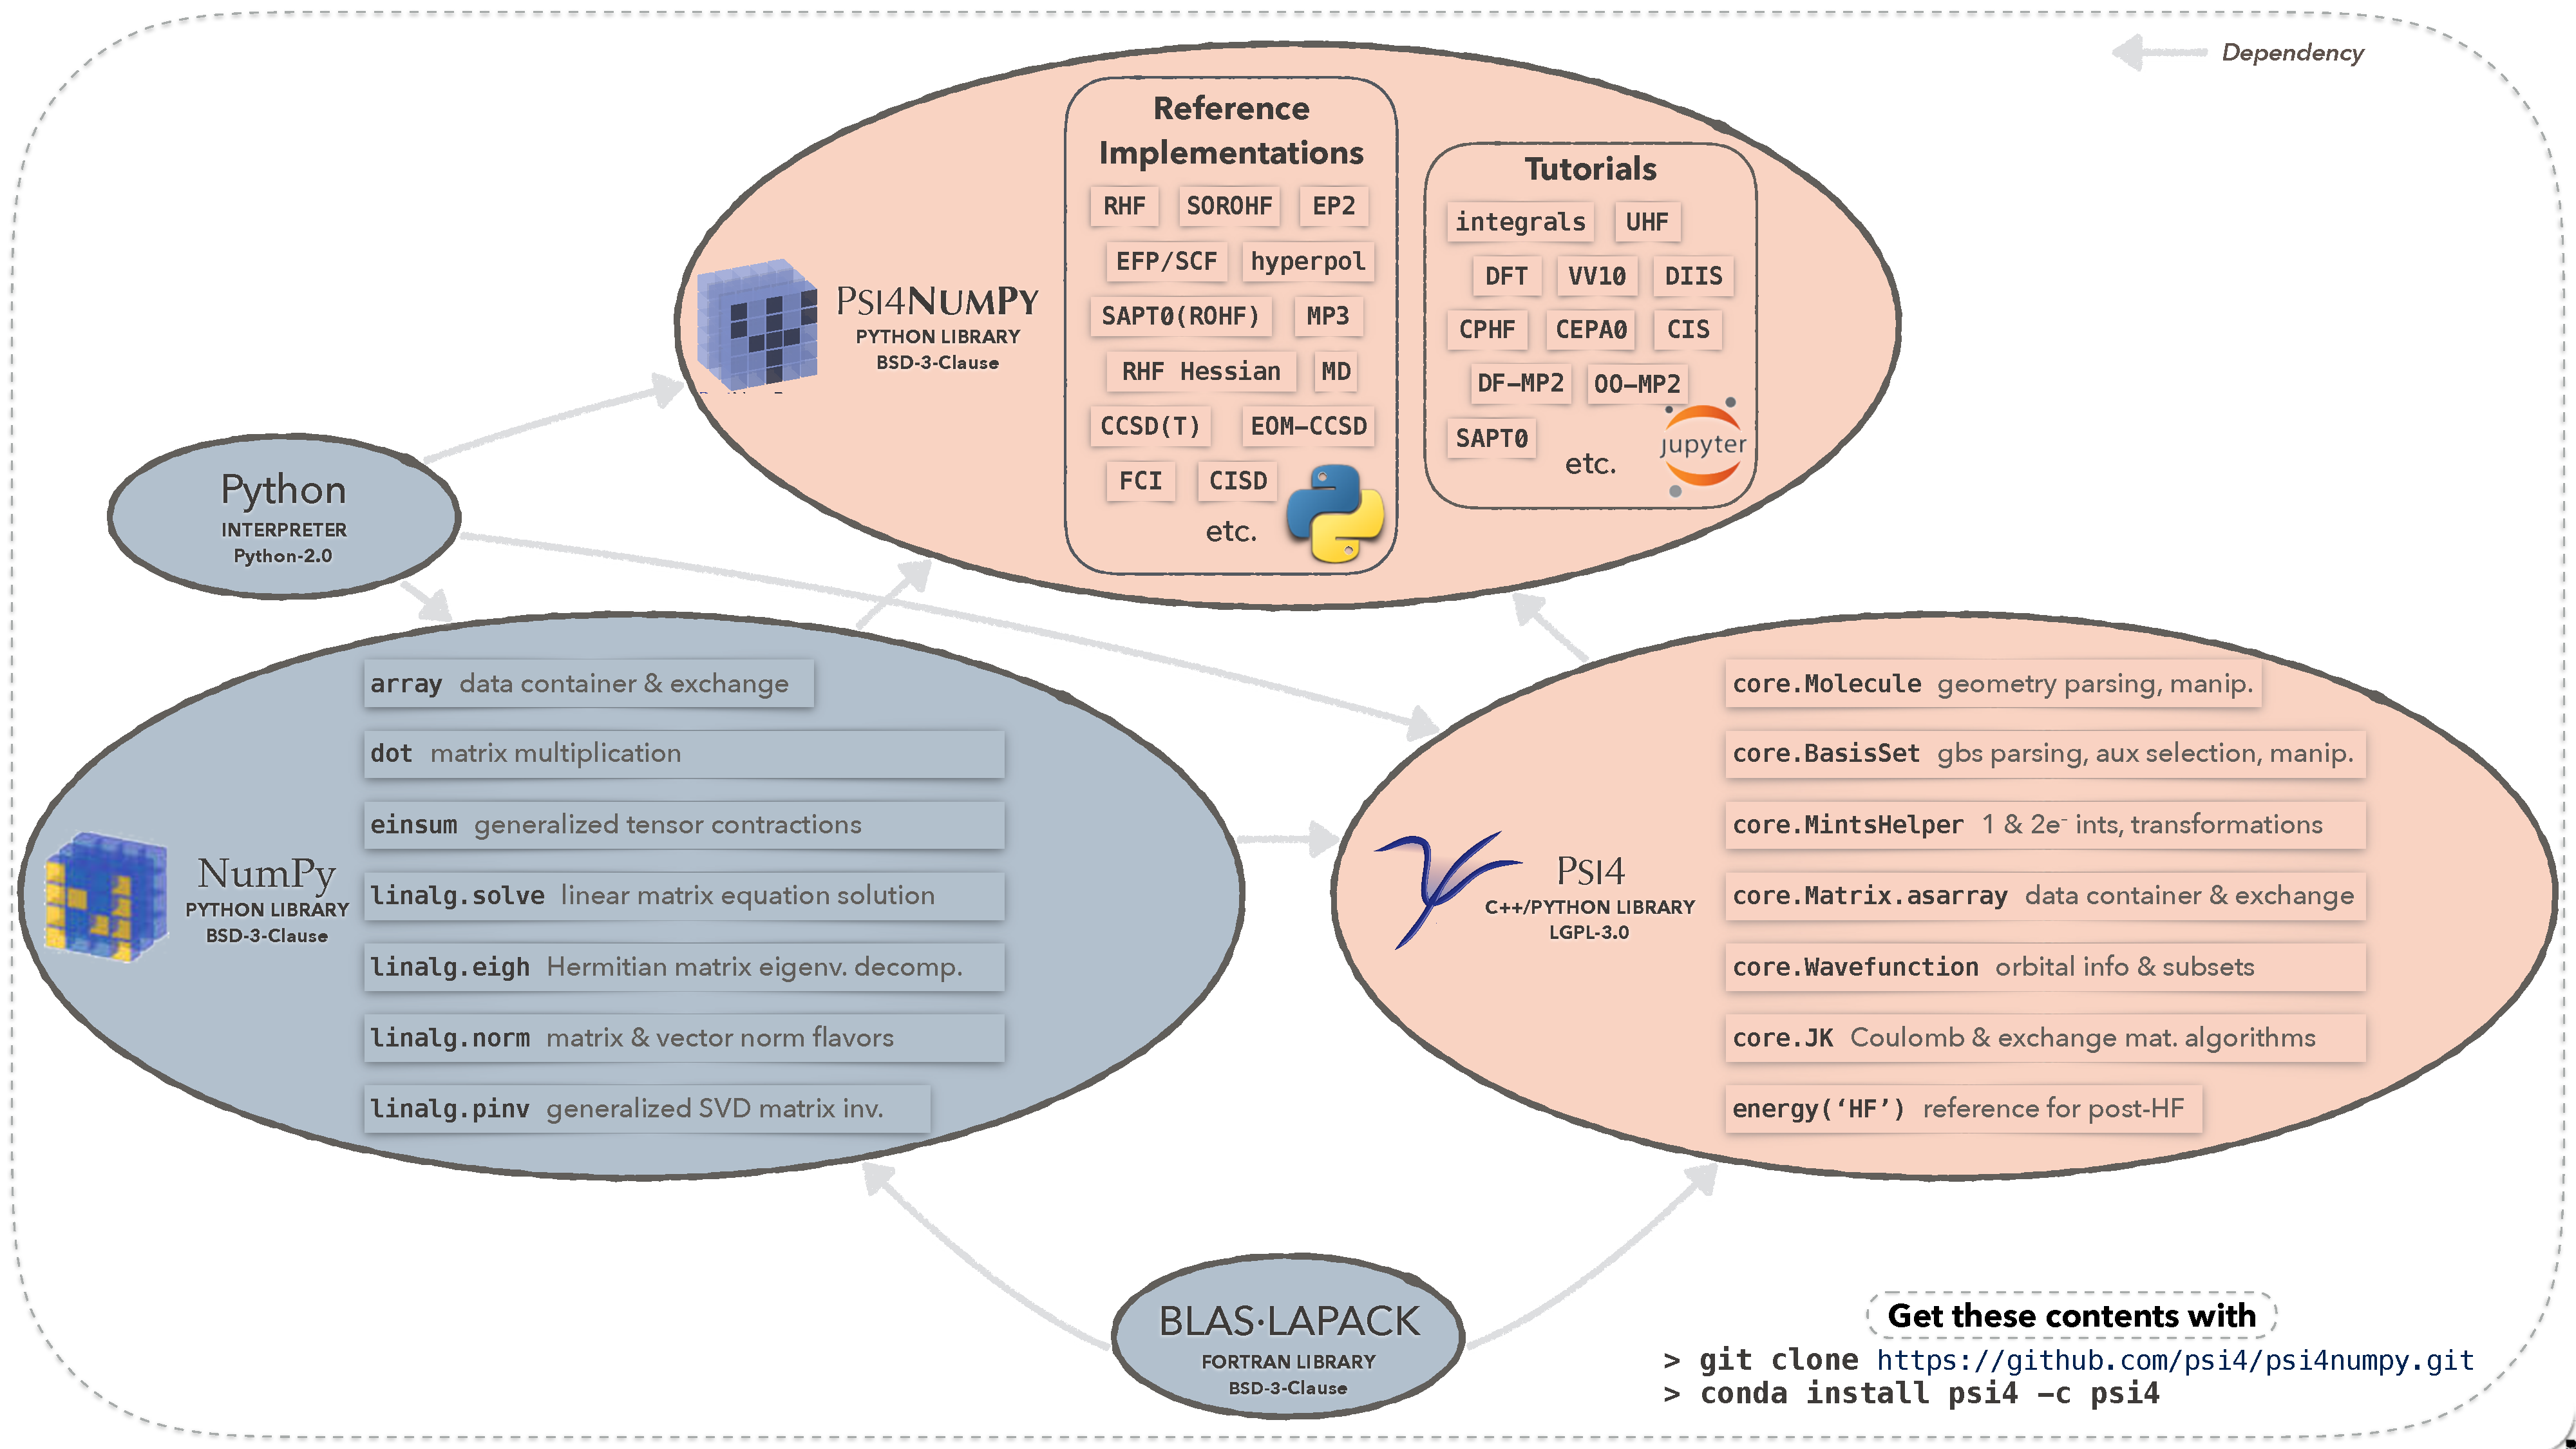
\includegraphics[width=\linewidth,keepaspectratio]{fig1-oval-org.pdf}
  \caption[Location of \pfn within the scientific computing ecosystem]{\pfn draws linear algebra tools from \numpy and fundamental quantum chemistry structures from \pfour to bring together a practical and convenient environment for code development, verification, and exploration. The most important data structures and functions are shown for \numpy and \pfour as well as representative tutorial and reference implementations presently in \pfn.}
  \label{fig:ovalorg}
\end{figure}

Shortly before submission, we discovered the Quantum Chemistry Program Exchange (QCPE)\cite{QCPE,Boyd:2013:221}, whose goals of (self-contained) software accessibility, algorithm explication, and free software ``publishing'' the \pfn project shares. The general tools embraced by \pfn (GitHub for communication, \numpy for linear algebra, Python for interfacing, and Jupyter for illumination) further allow rapid prototyping and educational objectives. In this manner \pfn can be thought as a modern successor to QCPE built to serve the flexible needs of the community.

\section{\texorpdfstring{\caps{Basic Tools}}{Basic Tools}}

The basic premise of \pfn is to leverage \pfour to generate quantum chemistry-specific quantities and the \numpy library\cite{Varoquaux:1521-9615} for all other tensor manipulations.  The latest version of \pfour has added the capability to import \pfour as a Python module as well as continuing to be called in an executable fashion. In this way, both the \pfour and \numpy libraries can be loaded into a single Python script and used in cooperation.

A key capacity in this enterprise is seamless translation between \numpy and \pfour data classes. For example, converting from a \numpy array to a \pfour matrix and back again can be easily accomplished:

\begin{minted}[label=snip:np2p42np]{python}
import numpy, psi4
np_array = numpy.zeros((5, 5))
psi4_matrix = psi4.core.Matrix.from_array(np_array)
new_np_array = numpy.array(psi4_matrix)
\end{minted}
At the core of this procedure is \textsc{NumPy}'s \arrayint \cite{array_interface} protocol, a basic specification for dense matrices consisting of
\begin{enumerate}
\item (a) the starting memory location for an in-memory array
\item (b) the overall ``shape'' of the array [\((n,)\) for a vector, \((n,m)\) for a matrix, etc.]
\item (c) the type of data involved (\texttt{double64}, \texttt{int32}, etc.)
\end{enumerate}
This specification is compact and widely used amongst the scientific Python community in a variety of scenarios. Using the \arrayint, it becomes straightforward to allow \numpy access to a \pfour data class, allowing both \pfour and \numpy to access and manipulate the same data. For example, the below will overwrite the \pfour Matrix class in place with a random \numpy array:

\begin{minted}[label=snip:numpy_set]{python}
psi4_matrix.np[:] = numpy.random.rand(5, 5)
\end{minted}
In this way the typical separation between general tensor frameworks and custom quantum chemistry data structures is removed.

A description of the full set of capabilities of the \arrayint is available in the \pfour documentation: \url{http://psicode.org/psi4manual/master/numpy.html}.

\subsection{Wavefunction Objects}

In \pfour all built-in methodologies have the option to return a Wavefunction object that holds basic information about the previous computation or, in some cases, holds functions for readily computing advanced quantities. Obtaining the Wavefunction object in this manner is straightforward:

\begin{minted}[label=snip:scf_computation]{python}
mol = psi4.geometry("""
O
H 1 0.96
H 1 0.96, 104.5
""")
hf_e, hf_wfn = psi4.energy("HF/cc-pVDZ", molecule=mol, return_wfn=True)
\end{minted}
Once a Wavefunction object is obtained, a variety of attributes can be queried
using standard Python syntax:

\begin{minted}[label=snip:wfn_data]{python}
# Number of doubly occupied orbitals
docc = hf_wfn.ndocc()
# Alpha orbital coefficient matrix
Ca = hf_wfn.Ca()
# Occupied subset of the alpha orbitals
Ca_occ = hf_wfn.Ca_subset("AO", "OCC")
\end{minted}
In addition to generating useful information after a computation, a Wavefunction object can also be passed as reference state to a further computation.  For \pfn, this means that reference implementations of post-Hartree--Fock methods (MPn, CCSD, etc.) need not re-code their own Hartree--Fock program; this simultaneously reduces code duplication and increases readability, both of which are cornerstones of the \pfn project.

% In particular, SCF Wavefunctions also have the ability to obtain SCF (Hartree-Fock) level quantities. For example, using a SCF Wavefunction one can "step" through the iterations by successively calling the Roothan-Hall equations:

% \begin{verbatim}
% form_C() # Forms the orbital matrix from the current Fock matrix
% form_D() # Forms the density matrix from the current orbital matrix
% form_F() # Forms the Fock matrix from the current density matrix.
% \end{verbatim}

% To better acquaint users with the Python-exposed functions of all Psi4 classes, use the built-in Python {\tt help} function. For example, using the above Wavefunction object:

%\begin{verbatim}
%>>> help(hf_wfn)
% |  Methods inherited from HF (Hartree-Fock):
% |  form_C(...) from builtins.PyCapsule
% |      form_C(self: psi4.core.HF) -> None
% |
% |      Forms the Orbital Matrices from the current Fock Matrices.
% |
% |  form_D(...) from builtins.PyCapsule
% |      form_D(self: psi4.core.HF) -> None
% |
% |      Forms the Density Matrices from the current Orbitals Matrices
%  ...
% |  Methods inherited from Wavefunction:
% |
% |  Ca(...) from builtins.PyCapsule
% |      Ca(self: psi4.core.Wavefunction) -> psi4.core.Matrix
% |
% |      Returns the Alpha Orbitals.
% |
% |  S(...) from builtins.PyCapsule
% |      S(self: psi4.core.Wavefunction) -> psi4.core.Matrix
% |
% |      Returns the One-electron Overlap Matrix.
%\end{verbatim}

\subsection{Integrals}

\pfour offers a wide selection of efficient C++ tools accessible directly in Python.  These tools are largely object-based and capable of storing quantities in memory or on disk.  One such object is the \texttt{libmints} library\cite{Psi41.1}, which is currently the primary interface for computing one- and two-electron integrals in \pfour.  This library is accessible through the \texttt{MintsHelper} class that directs the efficient computation and storage of molecular integrals Python-side:

\begin{minted}[label=snip:mints]{python}
# Create instance of MintsHelper using primary basis set
mints = psi4.core.MintsHelper(primary_basis)
# Compute one-electron AO overlap matrix
S = mints.ao_overlap()
# Compute core Hamiltonian matrix
T = mints.ao_kinetic()
V = mints.ao_potential()
H = T + V
# Compute two-electron integrals in AO basis in memory
I_ao = mints.ao_eri()
\end{minted}
Each of the above \texttt{MintsHelper} class methods returns a \pfour matrix which can be converted to a \numpy array using \texttt{numpy.asarray(matrix)} or modified in place with the \texttt{matrix.np} accessor.

In addition to computing molecular integrals, the \texttt{libmints} library also performs optimized electron repulsion integral (ERI) transformations. For example, the \(\mathcal{O}(N^5)\) transformation of the two-electron integrals between the atomic orbital and molecular orbital basis, given by
\begin{equation}
  (ia\vert jb) = \left[\left[C_{\mu i}\left[C_{\nu a}(\mu\nu\vert\lambda\sigma)\right]\right]C_{\lambda j}\right]C_{\sigma b},
  \label{eq:aomo}
\end{equation}
can be performed easily with:

\begin{minted}[label=snip:eri_trans]{python}
# Occupied and virtual subsets of SCF orbital coefficient matrices
Ca_occ = hf_wfn.Ca_subset("AO", "OCC")
Ca_virt = hf_wfn.Ca_subset("AO", "VIR")
# AO basis to MO basis in-memory ERI transform
I_mo = mints.mo_transform(Ca_occ, Ca_virt, I_ao, Ca_occ, Ca_virt)
\end{minted}
In this manner, arbitrary ERI transformations may be performed, allowing both speed and flexibility for constructing reference implementations.

\subsection{Coulomb and Exchange (JK) Matrix Objects}

A key component in SCF-level theories is the contraction of the 4-index electron repulsion integrals with the 2-index density matrix to form \(J\) and \(K\) matrices:
\begin{align}
  \label{eq:psi4numpy-coulomb}
  J_{\lambda \sigma}[D] &\equiv (\lambda\sigma|\mu\nu) D_{\mu\nu}, \\
  \label{eq:psi4numpy-exchange}
  K_{\lambda \sigma}[D] &\equiv (\lambda\mu|\sigma\nu) D_{\mu\nu}
\end{align}
\pfour provides objects for computing generalized Coulomb (J) and Exchange (K) matrices, with specialized algorithms for integral-direct, PK supermatrix\cite{20}, or density fitting (DF) scenarios.  For the DF-JK object, it is often advantageous to use a factorized form of the density matrix,
\begin{equation}
  D_{\mu\nu} \equiv C^\text{left}_{\mu p} C^\text{right}_{\nu p},
\end{equation}
where \(p\) is a general MO index. For example, in canonical Restricted Hartree Fock (RHF), the density matrix takes the form of
\begin{equation}
  D^{RHF}_{\mu\nu} = C_{\mu i} \chi_{ia} C_{\nu a},
\end{equation}
where \(i\) runs only over occupied orbitals. The computation of the RHF JK matrices can be translated directly to Python code with the following lines:

\begin{minted}[label=snip:jk]{python}
# Create a JK object in the current primary basis set
jk = psi4.core.JK.build(primary_basis)
# Add the occupied parts of the SCF orbital matrix
jk.add_C_left(C_occupied)
jk.add_C_right(C_occupied)
# Perform the computation and obtain the J and K matrices
jk.compute()
J = jk.J()
K = jk.K()
\end{minted}
In this fashion, virtually any SCF-level theory can be formulated at the \pfn layer by handling only 2-D arrays with \numpy (typically by threaded vendor BLAS) and leaving the 3- and 4-D arrays to \pfour libraries (using optimized C++ routines).  Thus, SCF-level theories can be implemented with the same efficiency as their pure C++ counterparts.

To illustrate this point, the \pfour SCF program is compared against a \pfn implementation on an Intel i7-5930K processor with the adenine\(\cdot\)thymine complex in the aug-cc-pVTZ basis (1127 basis functions) using a density-fitted JK build on six cores. The \pfour SCF program took 250 seconds while the \pfn implementation took 245 seconds. This should not be surprising as each spent 94\% total wall time computing the J and K quantities (both implementations used 18 SCF iterations) and all other operations of nonnegligible cost use the same BLAS implementations.

\section{\texorpdfstring{\caps{Rapid Development}}{Rapid Development}}

A key component of the \pfn framework is to provide an easy-to-use development environment for rapid prototyping. Vital to this is \numpy's \einsum function that performs arbitrary tensor contractions using Einstein summation syntax.  For example, the atomic orbital to molecular orbital 4-index transformation of Eq.~(\ref{eq:aomo}) and code snippet (\ref{snip:eri_trans}) could be accomplished by:

\begin{minted}[label=snip:aomo]{python}
I_mo = numpy.einsum("pi,qa,pqrs,rj,sb->iajb",
                    Ca_occ, Ca_virt, I_ao,
                    Ca_occ, Ca_virt)
\end{minted}
Recently, one of us (D.G.A.S.) modified \numpy's \einsum function so that it will automatically factorize the incoming tensor expression to reduce the cost of the operation from naive \(\mathcal{O}(N^8)\) to the conventional \(\mathcal{O}(N^5)\) version. This feature is available in \numpy 1.12 and onwards, with additional optimizations and BLAS usage occurring in \numpy 1.14. In addition, a drop-in replacement for the \einsum function, which makes optimal use of vendor BLAS, can be found through the Optimized Einsum project.\cite{danielsmith2016:160842}

Using the \einsum function, it is straightforward to transcribe existing equations directly into working code without a compilation stage.  While the resulting program is not as efficient for post-SCF level theories as a full implementation in a low-level language, the code is easy to read and modify without the need for compilation, allowing considerable flexibility when prototyping. In addition, the resulting program will provide correct answers for the given expressions, sparing the developer any worry whether low-level code is correct.

As an example of rapid prototyping, we use a temporary CCSD quantity in the Direct Product Decomposition formalism\cite{Bartlett1991:4334}. For virtual indices \(a, b, c, d\) and occupied indices \(i,j,k\), Equation 8 of Ref.~\parencite{Bartlett1991:4334} is written as:
\begin{equation}
  W_{jaci} = \langle ja || ci \rangle + t^d_i \langle ja || cd \rangle - t^a_k \langle jk || ci \rangle - (\frac{1}{2}t^{da}_{ik} + t^d_it^a_k) \langle jk || cd \rangle,
\end{equation}
which can be directly translated into a function:

\begin{minted}[label=snip:cc_example]{python}
def build_Wjaci(T1, T2, MO):
    Wjaci = MO[o, v, v, o].copy()
    Wjaci += numpy.einsum("jid,jacd->jaci", T1, MO[o, v, v, v])
    Wjaci -= numpy.einsum("ka,jkci->jaci", T1, MO[o, o, v, o])
    tmp = 0.5 * T2 + numpy.einsum("jid,ka->ikda", T1, T1)
    Wjaci -= numpy.einsum("ikda,jkcd->jaci, tmp, MO[o, o, v, v])
    return Wjaci
\end{minted}
Here, \texttt{MO} holds the 4-index antisymmetrized integrals, \texttt{T1} and \texttt{T2} the current amplitudes, and the \texttt{o, v} quantities are Python-based slices so that \texttt{MO[o, v, v, v]} returns the occupied-virtual-virtual-virtual blocks of the antisymmetrized integrals.

To our knowledge, the first implementations of Symmetry-Adapted Perturbation Theory with Complete Active Space SCF references [SAPT(CASSCF)], fourth-order Electron Propagator Theory, and transcorrelated theories have all been achieved using these rapid prototyping techniques.

\section{\texorpdfstring{\caps{Access and Contributions}}{Access and Contributions}}

To ensure ease of community access to the \pfn project, all software dependencies are made available as binary Conda packages\cite{ContinuumIO} either by us (e.g., \pfour), or by ContinuumIO or Intel (e.g., \numpy, Matplotlib, Jupyter). Through this route, binary distributions are installable in a single line to all common computing platforms, so users are not required to compile, link against the correct libraries, or debug runtime issues. We hope that the ready accessibility of these tools facilitates their use in methods development and in the creation of additional publicly available reference implementations.

To lower the barrier to contribution, guidance is included in the repository regarding attribution, citations, and testing. Though the authors adhere to Python software developement best practices in their other projects, they resist advanced Python syntax, organization, file linking, or other jargon-ized code in \pfn in favor of straightforward scripts and Jupyter notebooks for ease of community involvement.  Educators are encouraged to base lessons and labs off this work and are also referred to the \textsc{Psi4Education} project\cite{psi4edu}.

\section{\texorpdfstring{\caps{Reference Implementations}}{Reference Implementations}}

To illustrate the \pfn tools, and to provide a resource to the quantum chemistry methods development community, we have created a number of reference implementations and made them publicly available on GitHub at \url{https://github.com/psi4/psi4numpy}.  We intend to add to this collection over time.  Given the wide spectrum of quantum chemical methods, we also encourage submissions from other developers.

The \pfn reference implementations, while not necessarily as efficient as optimized versions in a low-level language, furnish at least the basic requirements for a programmer to reproduce the methodology. These references provide a medium to explain minute details that might be included in a corresponding paper and to record algorithmic tricks used to improve numerical stability or computational efficiency. In addition, these clear implementations will make explicit any important steps that might not be mentioned in a paper because they are assumed to be background knowledge in a given subfield of quantum chemistry.

Programmers can use these reference implementations to obtain intermediate quantities to validate a new implementation at every step, ensuring accuracy and assisting in the process of debugging a new program. These reference implementations can also be used as starting points for either building upon existing methodologies or exploring new methodologies in combination with the rapid prototyping aspects of this project.

Current reference implementations include
\begin{enumerate}
\item Self-Consistent Field
   \begin{enumerate}
   \item Restricted simple and DIIS\cite{25}-accelerated Hartree--Fock
   \item Restricted, Unrestricted, and Restricted Open-Shell Hartree--Fock
   \item Restricted, Unrestricted, and Restricted Open-Shell Hartree--Fock time-independent orbital Hessians
   \item Restricted time-dependent Hartree--Fock and coupled-perturbed Hartree--Fock for dipole polarizabilities
   \item Restricted nuclear gradients and Hessians
   \end{enumerate}

\item Many-Body Perturbation Theory
    \begin{enumerate}
    \item Canonical and density-fitted MP2
    \item Spin-integrated and spin-orbital MP3
    \item Arbitrary-order MP
    \end{enumerate}

\item Coupled-Cluster
    \begin{enumerate}
    \item Simple and DIIS-accelerated CCSD
    \item CCSD(T)
    \item CCSD dipole polarizabilities
    \item Time-dependent equation-of-motion CCSD
    \end{enumerate}

\item Configuration Interaction
    \begin{enumerate}
    \item Excited-state CIS
    \item Canonical and Davidson--Liu CISD
    \item Full configuration interaction
    \end{enumerate}

\item Symmetry-Adapted Perturbation Theory
    \begin{enumerate}
    \item Restricted and Restricted Open-Shell SAPT0
    \item Atomic orbital implementation of SAPT0
    \end{enumerate}

\item Electron Propagator Theory
    \begin{enumerate}
    \item Spin-integrated and spin-orbital EP2
    \item Spin-orbital EP3
    \end{enumerate}

\end{enumerate}

\subsection{Jupyter Notebook integration}

As a service to the community, some of the reference implementations have been augmented by additional, tutorial-style background information on various subfields of quantum chemistry.  We found it convenient to add this additional information using the Jupyter notebook web application,\cite{Granger:1521-9615} a popular Integrated Development Environment (IDE) for interactive computing in several programming languages that is starting to be adopted by chemists \cite{charles:2017:592}.  An example for restricted Hartree--Fock can be found in Fig.~\ref{fig:ipython}.

\begin{figure}
  \centering
  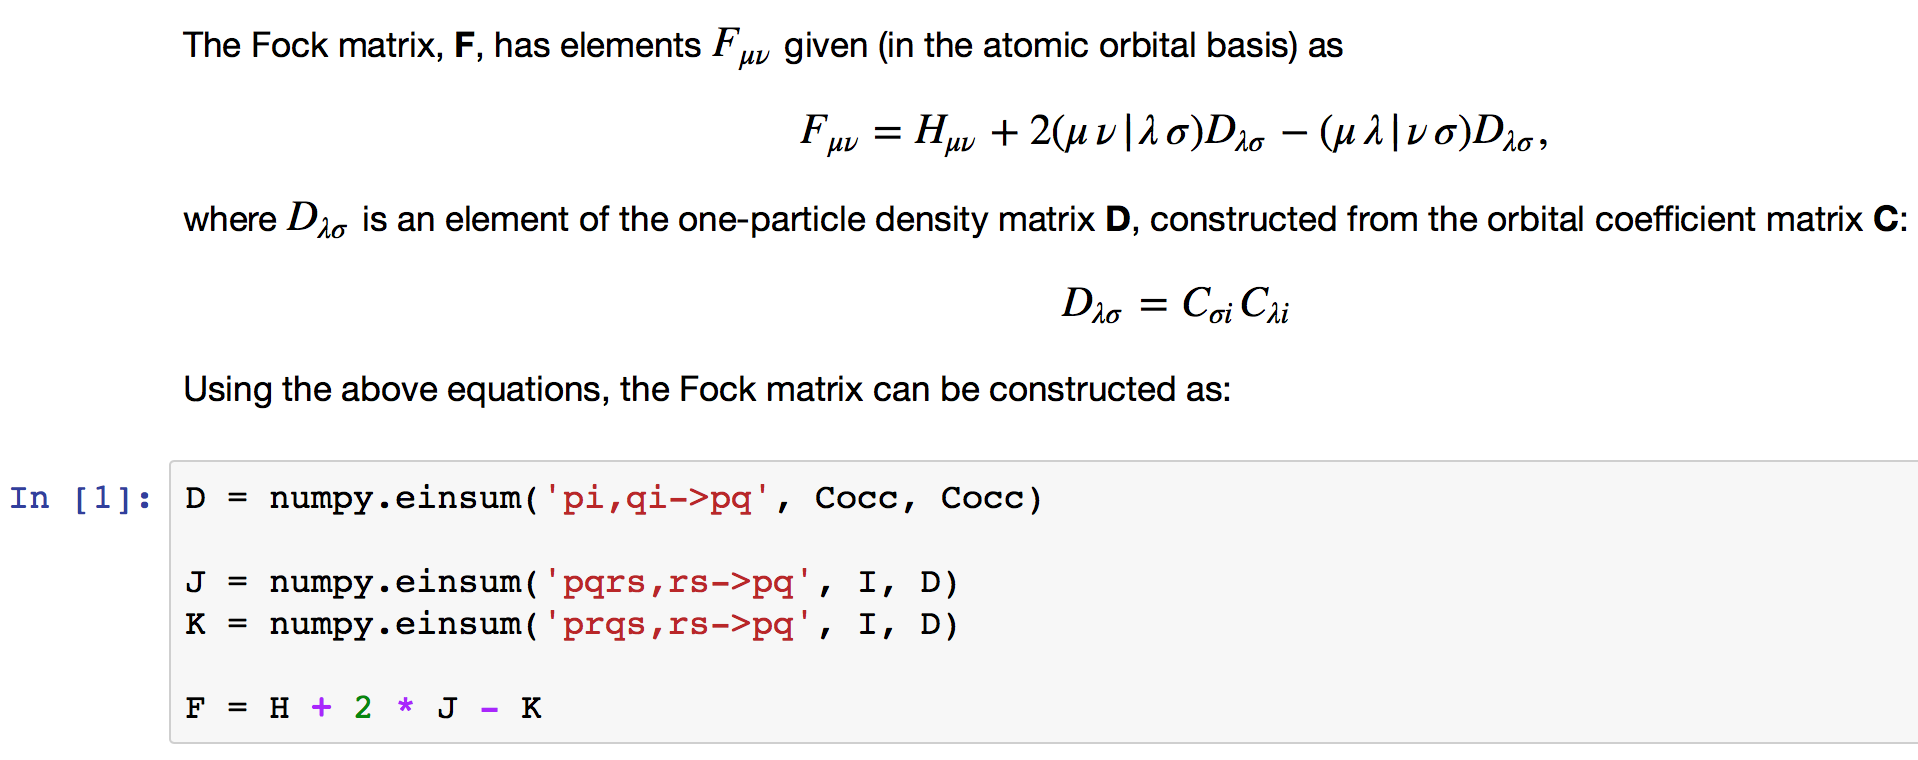
\includegraphics[width=\linewidth,keepaspectratio]{fig2-ipython-rhf.png}
  \caption[Extract from a \pfn tutorial notebook]{Extract from a Jupyter notebook demonstrating the construction of a SCF Fock matrix where \texttt{I} is the 4-index electron repulsion integral array and \texttt{Cocc} is the occupied orbital matrix.}
  \label{fig:ipython}
\end{figure}

These documents may be unique within quantum chemistry in that they focus not only on theoretical considerations but also on the details of a method's implementation, such as \emph{why} certain programming choices were made. For example, the comparison between a general matrix inversion and solving a set of linear equations demonstrates instability issues that often plague the former technique. Such illustrations should make the Jupyter implementations useful both to new users in quantum chemistry and to experienced users interested in exploring new subfields.

Current tutorial-style Jupyter reference implementations include

\begin{enumerate}
\item Introductions to the \pfn methodology
\item Introduction to Hartree--Fock, DIIS, and density fitting
\item Density Functional Theory: grids, LDA kernels, VV10 dispersion, and asymptotic corrections
\item M\o ller--Plesset: canonical and density-fitted reference implementations of MP2
\item Molecular Properties: Integrals, CPHF, CIS
\item Symmetry-Adapted Perturbation Theory: Canonical and atomic orbital algorithms
\item Orbital-Optimized Methods: OMP2
\item Coupled-Cluster Approximations: CEPA0, CCD
\item  Geometry Optimization Techniques: Internal Coordinates, Hessian guesses, and advanced Newton-Raphson methods
\end{enumerate}
Molecular-dynamics tutorials include
\begin{enumerate}
\item Periodic Lennard-Jones simulation with Verlet integrators
\item Periodic Ewald Electostatic summation
\end{enumerate}

\section{\texorpdfstring{\caps{Conclusions}}{Conclusions}}

We believe that the benefits of the \pfn framework to the computational chemistry community are threefold.  Beginning researchers can use the \pfn reference implementations for \emph{education}. Reference implementations convey not just the underlying mathematical formulas of a given theory, but how to implement these formulas in a manner that avoids common pitfalls such as ill-conditioned numerical equations. \pfn is likely the most interactive educational resource available in this field: thanks to the Jupyter Notebook format, the learners can explore the implementation step by step and easily try out various modifications and additional approximations.

More advanced researchers who need to reimplement and/or modify a given computational chemistry approach can use the \pfn reference implementations for \emph{validation}, taking advantage of the code that, thanks to the extensive use of the \numpy \einsum functionality, provides a nearly one-to-one correspondence between the terms in a formula and the lines of Python code. As a result, it is trivial to switch off, for debugging purposes, any subset of terms as well as generate an arbitrary intermediate without even recompiling any code.  This feature should be contrasted with the situation when one tries to validate their code against a C++/Fortran implementation from an established electronic-structure package. Once the relevant fragment of code that does the actual computation is found (which is not always trivial), various terms are typically combined in nontrivial ways to improve computational performance. As a result, getting out a specific intermediate for checking the implementation in progress often requires substantive changes to the reference code, not to mention its recompilation.  In addition, we include the programmed formulas together with their implementation in the Jupyter Notebook to alleviate difficulties associated with incompatible notation or even errors in the originally published expressions.

Finally, for researchers who want to develop new functionality, \pfn is a highly valuable platform for \emph{initial implementation} that is efficient enough for meaningful testing, quick to generate, easy to debug, and has few opportunities for programming errors. All underlying quantum-chemistry building blocks such as integrals, orbitals, density matrices, and CI vectors are efficiently computed by \pfour and readily imported in the \numpy format. In particular, a \pfn implementation of any one-electron theory such as HF or DFT is already close to optimal as the most expensive operations are all written in terms of generalized Coulomb and exchange matrices which are supplied by \pfour.  Some of us, together with their collaborators, have already taken advantage of the \pfn capabilities to rapidly generate pilot implementations of brand new electronic-structure approaches.

\section{\texorpdfstring{\caps{Acknowledgements}}{Acknowledgements}}

This work was supported in part by the U.S.~National Science Foundation through grants ACI-1449723 and CHE-1566192 for D.G.A.S, L.A.B., D.A.S, and C.D.S; CHE-1661604 for B.Z., A.S.A, J.M.T., and H.F.S; CHE-1554354 for D.R.N and A.E.D. B. Z. contributions to this work were also supported by a Software Fellowship from the Molecular Sciences Software Institute, which is funded by the U.S. National Science Foundation (ACI-1547580). M.H.L. acknowledges financial support by the Studienstiftung des Deutschen Volkes. K.P. is supported by the U.S. National Science Foundation CAREER award CHE-1351978.

\section{\texorpdfstring{\caps{Supporting Information}}{Supporting Information}}

Documents reproducing all currently available reference implementations and interactive tutorials are available free of charge via the Internet at \url{https://zenodo.org/record/1134320}. For all future materials, please see \url{https://github.com/psi4/psi4numpy}. The code found in sections~\ref{paper_05:ssec:hyperpolarizability_reference_implementation}~and~\ref{paper_05:ssec:hyperpolarizability_tutorial} was merged in commit hash \href{https://github.com/psi4/psi4numpy/tree/066f378f26240a4802371ef32849230853581329}{066f378}.

\subsection{Hyperpolarizability Reference Implementation}
\label{paper_05:ssec:hyperpolarizability_reference_implementation}

\begin{singlespace}
\inputminted[escapeinside=||]{python}{\IfStandalone{helper_CPHF.py}{paper_05/helper_CPHF.py}}
\inputminted{python}{\IfStandalone{beta.py}{paper_05/beta.py}}
\end{singlespace}

\subsection{Hyperpolarizability Tutorial}
\label{paper_05:ssec:hyperpolarizability_tutorial}

\providecommand{\tightlist}{%
  \setlength{\itemsep}{0pt}\setlength{\parskip}{0pt}}
\IfStandalone{\begin{minted}[]{python}
"""Tutorial: SCF first hyperpolarizability"""

__author__    = "Eric J. Berquist"
__credit__    = ["Eric J. Berquist"]

__copyright__ = "(c) 2014-2017, The Psi4NumPy Developers"
__license__   = "BSD-3-Clause"
__date__      = "2017-12-19"
\end{minted}

\hypertarget{scf-first-hyperpolarizability}{%
  \section{SCF First Hyperpolarizability}\label{scf-first-hyperpolarizability}}

\hypertarget{introduction}{%
  \subsection{Introduction}\label{introduction}}

In Tutorial 6a, the calculation of linear response properties from analytic derivative theory is presented, the foundation of which are the coupled-perturbed Hartree-Fock (CPHF) or coupled-perturbed self-consistent field (CPSCF) equations. Starting from analytic derivative theory provides a convenient physical picture: how does the total energy of a system change under the influence of one or more internal or external perturbations? Continuing the case of an external electric field, the total energy of a system can be represented with a series expansion:
\begin{equation}
  E(\mathbf{E}) = \sum_{n=0}^{\infty} \frac{1}{n!}E^{(n)}(\mathbf{a})\cdot(\mathbf{E}-\mathbf{a})^{n},
\end{equation}
where the electric field is \(\mathbf{E} = \vec{E} = (E_x,E_y,E_z)\) and \(\mathbf{a}\) is the expansion point. In practice, we always expand around \(\mathbf{a} = \mathbf{0}\), so it is a Maclaurin series:
\begin{equation}
  E(\mathbf{E}) = \sum_{n=0}^{\infty} \frac{1}{n!}\mathbf{E}^{(n)}(\mathbf{0})\cdot\mathbf{E}^{n}.
\end{equation}
Expanding the above to the first 4 explicit terms gives
\begin{equation}
  E(\mathbf{E}) \approx E^{(0)}(\mathbf{0}) + \mathbf{E}^{(1)}(\mathbf{0})\cdot\mathbf{E} + \frac{1}{2}\mathbf{E}^{(2)}(\mathbf{0})\cdot\mathbf{E}^{2} + \frac{1}{6}\mathbf{E}^{(3)}(\mathbf{0})\cdot\mathbf{E}^{3},
\end{equation}
where we identify
\begin{align}
E^{(0)} &\rightarrow \textrm{the unperturbed ground-state energy} \\
E_{a}^{(1)} &\rightarrow -\mu_{a},\textrm{the dipole moment} \\
E_{ab}^{(2)} &\rightarrow -\alpha_{ab},\textrm{the polarizability} \\
E_{abc}^{(3)} &\rightarrow -\beta_{abc},\textrm{the first hyperpolarizability}
\end{align}
The first hyperpolarizability is the leading-order term that describes the \emph{nonlinear} response of a system to an external electric field.  Each term in the series expansion increases the rank of the coefficient by one: the ground-state energy is a scalar, the dipole is a length 3 vector, the polarizability is a 3-by-3 matrix, and the first hyperpolarizability is a 3-by-3-by-3 tensor.

Translated into the language of analytic derivative theory, is it represented as
\begin{equation}
  \beta_{abc} = \left.\frac{\partial^{3} E}{\partial E_a \partial E_b \partial E_c}\right|_{\mathbf{E}=\mathbf{0}},
\end{equation}
though it is not yet clear how to take derivatives of the energy beyond what is presented in tutorial 6a. Additionally, nothing has been stated about time dependence; everything to this point has been the static case, where the strength of fields do not vary with time. We will first incorporate time dependence, and equations for derivative theory will result.

\hypertarget{notation}{%
  \subsubsection{Notation}\label{notation}}

Before going further, some notational conventions should be mentioned.  When used as field indices, \(a,b,c,\dots \in \{x,y,z\}\), the three Cartesian directions.

For matrix indices, \(\mu,\nu,\lambda,\sigma,\dots\) label atomic orbitals (AOs)/basis functions, \(i,j,k,l,\dots\) label occupied molecular orbitals (MOs), \(a,b,c,d,\dots\) label unoccupied/virtual MOs, and \(p,q,r,s,\dots\) label all MOs. Einstein summation is used, so repeated indices are contracted over.

\hypertarget{derivation}{%
  \subsection{Derivation}\label{derivation}}

Again, write the total Hamiltonian as the sum of unperturbed and perturbed components
\begin{align*}
  \hat{H}(\mathbf{E},t) &= \hat{H}^{(0)} + \hat{V}(\mathbf{E},t) \\
  \hat{V}(\mathbf{E},t) &= -\mathbf{\mu} \cdot \mathbf{E}(e^{\pm i \omega t} + 1) \tag{Karna 2}
\end{align*}
where part of the external field now oscillates with some characteristic frequency \(\omega\). This can be incorporated into the time-dependent Schrodinger equation, which for a stationary state obeys
\begin{align*}
  \left[ \hat{H}^{(0)} + \hat{V}(\mathbf{E},t) - i\frac{\partial}{\partial t} \right] \psi(t) &= 0, \tag{Karna 3} \\
  FC - i \frac{\partial}{\partial t} SC &= SC\epsilon, \tag{Karna 5} \\
  \frac{\partial}{\partial t} C^{\dagger} S C &= 0, \tag{Karna 6}
\end{align*}
where the full definition of the Fock matrix is
\begin{equation}
  F_{\mu\nu} = h_{\mu\nu} + D_{\lambda\sigma}[2J_{\mu\nu\lambda\sigma} - K_{\mu\nu\lambda\sigma}] \tag{Karna 9}
\end{equation}
and the density matrix is defined as
\begin{equation}
  D_{\mu\nu} = C_{\mu p}n_{pq}C_{\nu q}^{\dagger}, \tag{Karna 10}
\end{equation}
where the diagonal occupation number matrix \(n_{ii} = 2\) and \(n_{aa} = 0\) for RHF.

In general, the MO coeffients are perturbation- and time-dependent, but the basis functions themselves are not. This means that when the series expansion for the perturbation above is performed on other quantities, only \(F\), \(C\), \(\epsilon\), and \(D\) are affected. For example, the Lagrangian multiplier matrix \(\epsilon\) can be expanded as
\begin{equation}
  \epsilon(\mathbf{E}) = \epsilon^0 + E_a\epsilon^a + \frac{1}{2!}E_aE_b\epsilon^{ab} + \frac{1}{3!}E_aE_bE_c\epsilon^{abc} + \cdots \tag{Karna 17c}
\end{equation}
where \(a,b,c,...\in\{x,y,z\}\), and
\begin{align*}
  \epsilon^{a} &= e^{\pm i \omega t} \epsilon^{a}(\pm\omega) + \epsilon^{a}(0), \tag{Karna 19a} \\
  \epsilon^{ab} &= e^{\pm 2 i \omega t} \epsilon^{ab}(\pm\omega,\pm\omega) + e^{\pm i \omega t} \{ \epsilon^{ab}(0,\pm\omega) + \epsilon^{ab}(\pm\omega,0)\} + \epsilon^{ab}(\pm\omega,\mp\omega) + \epsilon^{ab}(0,0), \tag{Karna 19b}
\end{align*}
\begin{equation}
  \begin{split}
    \epsilon^{abc} &= e^{\pm 3 i \omega t} \epsilon^{abc}(\pm\omega,\pm\omega,\pm\omega) + e^{\pm 2 i \omega t} \{\epsilon^{abc}(0,\pm\omega,\pm\omega) + \epsilon^{abc}(\pm\omega,0,\pm\omega) + \epsilon^{abc}(\pm\omega,\pm\omega,0)\} \\
    &+ e^{\pm i \omega t} \{\epsilon^{abc}(\pm\omega,\pm\omega,\mp\omega) + \epsilon^{abc}(\pm\omega,\mp\omega,\pm\omega) + \epsilon^{abc}(\mp\omega,\pm\omega,\pm\omega)\} \\
    &+ e^{\pm i \omega t} \{\epsilon^{abc}(0,0,\pm\omega) + \epsilon^{abc}(0,\pm\omega,0) + \epsilon^{abc}(\pm\omega,0,0)\} \\
    &+ \{\epsilon^{abc}(0,\pm\omega,\mp\omega) + \epsilon^{abc}(\pm\omega,0,\mp\omega) + \epsilon^{abc}(\pm\omega,\mp\omega,0)\} + \epsilon^{abc}(0,0,0),
  \end{split} \tag{Karna 19c}
\end{equation}
showing that each order of the expansion consists of all possible phase combinations. For the first hyperpolarizability, only quantities with at most two field indices are required. Each permutationally unique subterm of the expansion corresponds to a different physical observable:
\begin{align*}
  (0) \rightarrow \text{static polarizability} &\rightarrow \alpha(0;0) = -Tr[H^{a} D^{b}(0)] \tag{Karna IV-1a} \\
  (\pm\omega) \rightarrow \text{dynamic polarizability} &\rightarrow \alpha(\mp\omega;\pm\omega) = -Tr[H^{a} D^{b}(\pm\omega)] \tag{Karna IV-1b} \\
  (0,0) \rightarrow \text{static (first) hyperpolarizability} &\rightarrow \beta(0;0,0) = -Tr[H^{a} D^{bc}(0,0)] \tag{Karna IV-2a} \\
  (0,\pm\omega) \rightarrow \text{electrooptic Pockels effect (EOPE)} &\rightarrow \beta(\mp \omega;0,\pm\omega) = -Tr[H^{a} D^{bc}(0,\pm\omega)] \tag{Karna IV-2b} \\
  (\pm\omega,\pm\omega) \rightarrow \text{second harmonic generation (SHG)} &\rightarrow \beta(\mp 2\omega;\pm\omega,\pm\omega) = -Tr[H^{a} D^{bc}(\pm\omega,\pm\omega)] \tag{Karna IV-2c} \\
  (\pm\omega,\mp\omega) \rightarrow \text{optical rectification} &\rightarrow \beta(0;\pm\omega,\mp\omega) = -Tr[H^{a} D^{bc}(\pm\omega,\mp\omega)] \tag{Karna IV-2d}
\end{align*}
where each property is calculated as the trace over the AO-basis dipole matrices \(H^{a}\) with the appropriate perturbed density. The task now comes down to calculating the necessary perturbed density for the phenomenon of interest. The second-order densities required for the four different first hyperpolarizabilities are
\begin{align*}
  \begin{split}
    D^{ab}(\pm\omega,\pm\omega) &= C^{ab}(\pm\omega,\pm\omega) n C^{0\dagger} + C^{a}(\pm\omega) n C^{b\dagger}(\mp\omega) \\
    &+ C^{b}(\pm\omega) n C^{a\dagger}(\mp\omega) + C^{0} n C^{ab\dagger}(\mp\omega,\mp\omega),
  \end{split} \tag{Karna III-2a} \\
  \begin{split}
    D^{ab}(0,\pm\omega) &= C^{ab}(0,\pm\omega) n C^{0\dagger} + C^{a}(0) n C^{b\dagger}(\mp\omega) \\
    &+ C^{b}(\pm\omega) n C^{a\dagger}(0) + C^{0} n C^{ab\dagger}(0,\mp\omega),
  \end{split} \tag{Karna III-2b} \\
  \begin{split}
    D^{ab}(\pm\omega,\mp\omega) &= C^{ab}(\pm\omega,\mp\omega) n C^{0\dagger} + C^{a}(\pm\omega) n C^{b\dagger}(\pm\omega) \\
    &+ C^{b}(\mp\omega) n C^{a\dagger}(\mp\omega) + C^{0} n C^{ab\dagger}(\mp\omega,\pm\omega),
  \end{split} \tag{Karna III-2c} \\
  \begin{split}
    D^{ab}(0,0) &= C^{ab}(0,0) n C^{0\dagger} + C^{a}(0) n C^{b\dagger}(0) \\
    &+ C^{b}(0) n C^{a\dagger}(0) + C^{0} n C^{ab\dagger}(0,0).
  \end{split} \tag{Karna III-2d}
\end{align*}
Already a few important insights about the equations are revealed: Each perturbation index always carries its respective frequency, and the positive and negative frequencies are related by the Hermitian adjoint (except for \(C(-\omega) = -C^{0} U^{\dagger}(+\omega)\), Karna eq. 40).  We also see the appearance of terms like \(C^{ab}\), which will require \(U^{ab}\) originating from the second-order CPHF. Computationally, this is undesirable due to the increased number of iterative calculations that must be performed, so we borrow a trick that most prominently appears in perturbation theory.

\hypertarget{wigners-2n-1-rule}{%
  \subsubsection{\texorpdfstring{Wigner's \(2n + 1\) rule}{Wigner's 2n + 1 rule}}\label{wigners-2n-1-rule}}

From Schaefer\cite{Yamaguchi1994}, page 25:
\begin{quote}
  When the wavefunction is determined up to the \(n\)th order, the expectation value (electronic energy) of the the system is resolved, according to the results of perturbation theory, up to the \((2n+1)\)st order. This principle is called Wigner's \(2n+1\) theorem\cite{doi:10.1063/1.1668053,EPSTEIN1980311}.
\end{quote}
\begin{table}
  \centering
  \caption[MO coefficient derivatives and rotation matrices needed for energy derivatives]{Orders of MO coefficient derivatives and rotation matrices needed for energy derivatives following Wigner's \(2n+1\) rule. Reproduced from Ref.~\parencite{Yamaguchi1994}.}
  \label{tutorial:tab:wigner}
  \begin{tabular}{cccc}
    \toprule
    & CI: MO/CI space & MCSCF: MO/CI space & RHF: MO space \\
    \midrule
    Energy, \(E\) & \(C_{\mu}^{i}\), \(C_{I}\) & \(C_{\mu}^{i}\), \(C_{I}\) & \(C_{\mu}^{i}\) \\
    First Derivative, \(\frac{\partial E}{\partial a}\) & \(U^{a}\), \(C_{I}\) & \(C_{\mu}^{i}\), \(C_{I}\) & \(C_{\mu}^{i}\) \\
    Second Derivative, \(\frac{\partial^{2} E}{\partial a \partial b}\) & \(U^{ab}\), \(\frac{\partial C_{I}}{\partial a}\) & \(U^{a}\), \(\frac{\partial C_{I}}{\partial a}\) & \(U^{a}\) \\
    Third Derivative, \(\frac{\partial^{3} E}{\partial a \partial b \partial c}\) & \(U^{abc}\), \(\frac{\partial C_{I}}{\partial a}\) & \(U^{a}\), \(\frac{\partial C_{I}}{\partial a}\) & \(U^{a}\) \\
    Fourth Derivative, \(\frac{\partial^{4} E}{\partial a \partial b \partial c \partial d}\) & \(U^{abcd}\), \(\frac{\partial^{2} C_{I}}{\partial a \partial b}\) & \(U^{ab}\), \(\frac{\partial^{2} C_{I}}{\partial a \partial b}\) & \(U^{ab}\) \\
    Fifth Derivative, \(\frac{\partial^{5} E}{\partial a \partial b \partial c \partial d \partial e}\) & \(U^{abcde}\), \(\frac{\partial^{2} C_{I}}{\partial a \partial b}\) & \(U^{ab}\), \(\frac{\partial^{2} C_{I}}{\partial a \partial b}\) & \(U^{ab}\) \\
    \bottomrule
  \end{tabular}
\end{table}
Since the first hyperpolarizability is calculated as a third derivative of the energy, perturbed coefficients with only one field index should be required. From table~\ref{tutorial:tab:wigner}, we can also see why SCF gradients (\(\frac{\partial E}{\partial R_A}\), where \(R_A\) is the \(A\)-th Cartesian component of nucleus \(R\)) avoid the need to solve for \(U\) matrices.

\hypertarget{final-expressions}{%
  \subsection{Final expressions}\label{final-expressions}}

To this point, most work has been in the AO basis, but it is conceptually easier to work in the MO basis, in particular due to the use of the \(\epsilon\) equations
\begin{equation}
  \epsilon^{a}(\pm\omega) = G^{a}(\pm\omega) + \epsilon^{0} U^{a}(\pm\omega) - U^{a}(\pm\omega) \epsilon^{0} \pm \omega U^{a}(\pm\omega), \tag{Karna 34}
\end{equation}
where the \(G\) matrices are the MO-basis Fock matrices
\begin{equation}
  G^{ab\dots} = C^{0\dagger} F^{ab\dots} C^{0},
\end{equation}
and the \(U\) matrices are the MO-basis perturbation parameters
\begin{equation}
  C^{ab\dots} = C^{0} U^{ab\dots},
\end{equation}
which will be discussed in the implementation. The final expression for the static hyperpolarizability is
\begin{equation}
  \begin{split}
    \beta_{abc}(0; 0, 0) &= Tr[n \{U^{a}(0) G^{b}(0) U^{c}(0) + U^{c}(0) G^{b}(0) U^{a}(0) + U^{b}(0) G^{c}(0) U^{a}(0) \\
    &+ U^{a}(0) G^{c}(0) U^{b}(0) + U^{c}(0) G^{a}(0) U^{b}(0) + U^{b}(0) G^{a}(0) U^{c}(0)\} ] \\
    &- Tr[n \{ U^{a}(0) U^{c}(0) \epsilon^{b}(0) + U^{c}(0) U^{a}(0) \epsilon^{b}(0) + U^{b}(0) U^{a}(0) \epsilon^{c}(0) \\
    &+ U^{a}(0) U^{b}(0) \epsilon^{c}(0) + U^{c}(0) U^{b}(0) \epsilon^{a}(0) + U^{b}(0) U^{c}(0) \epsilon^{a}(0) \} ].
  \end{split} \tag{Karna VII-4}
\end{equation}
By noticing that each term corresponds to a unique permutation of the field indices, it can be rewritten as
\begin{equation}
  \beta_{abc} = Tr\left[ n \sum \mathcal{P}(d,e,f) U^{d} G^{e} U^{f} \right] - Tr\left[ n \sum \mathcal{P}(d,e,f) U^{d} U^{e} \epsilon^{f} \right],
\end{equation}
where the permutation indices are initially assigned as \(d = a, e = b, f = c\). The frequency notation has also been dropped, since each \(abc\) (and therefore each \(def\)) will always carry the appropriate field index, making this the most general form of the first hyperpolarizability. If the indices \(abc\) are also permuted, then all 27 components of the first hyperpolarizability tensor will be computed.

\hypertarget{computational-procedure}{%
  \subsection{Computational Procedure}\label{computational-procedure}}

The basic quantities we need are the matrices \(C, \mu, F, \epsilon\), and \(U\). The MO coefficients \(C\) are already obtained from the ground-state calculation, along with \(\epsilon^{0}\) (the MO energies) and \(F^{0}\) (the AO-basis Fock matrix). The dipole matrices \(\mu\) are needed for the linear response (polarizability) calculation, which results in response vectors that compose the off-diagonal blocks of the \(U^{a}\) matrix. \(G^{a}\) is obtained from \(F^{a}\), which comes from performing a single Fock build with the perturbed density \(D^{a}\).  Finally, \(\epsilon^{a}\) can be constructed.

Although the expressions so far are general for any frequency and first-order non-linear optical response, the tutorial implementation will cover the static case. For second-harmonic generation, see the reference implementation.

\begin{minted}[]{python}
import numpy as np
np.set_printoptions(3, linewidth=100, suppress=True)    # when we inspect the vectors/matrices,
                                                        # use a prettier format for printing
import psi4
\end{minted}
The energy and density convergence criteria are tightened from defaults, as response properties are sensitive to the quality of the ground-state wavefunction.

\begin{minted}[]{python}
mol = psi4.geometry('''
    O
    H  1  0.9435
    H  1  0.9435  2  105.9443
    symmetry c1
''')
psi4.set_options({
    "basis": "aug-cc-pVDZ",
    "scf_type": "direct",
    "df_scf_guess": False,
    "e_convergence": 1e-9,
    "d_convergence": 1e-9,
})
\end{minted}
\begin{minted}[]{python}
# This is to enable testing outside of the notebook environment.
import sys
try:
    get_ipython()
    sys.path.append('../../Response-Theory/Self-Consistent-Field')
except NameError:
    import os.path
    dirname = os.path.dirname(os.path.abspath(__file__))
    sys.path.append(os.path.join(dirname, '../../Response-Theory/Self-Consistent-Field'))

from helper_CPHF import helper_CPHF
\end{minted}
The helper encapsulates the solution of the ground-state wavefunction followed by the frequency\textendash{}(in)dependent linear response equations,
\begin{equation}
  \left[
    \begin{pmatrix}
      \mathbf{A} & \mathbf{B} \\
      \mathbf{B}^{*} & \mathbf{A}^{*}
    \end{pmatrix}
    - \omega_{f}
    \begin{pmatrix}
      \mathbf{\Sigma} & \mathbf{\Delta} \\
      -\mathbf{\Delta}^{*} & -\mathbf{\Sigma}^{*}
    \end{pmatrix}
  \right]
  \begin{pmatrix}
    \mathbf{X} \\
    \mathbf{Y}
  \end{pmatrix}
  =
  \begin{pmatrix}
    \mathbf{V} \\
    -\mathbf{V}^{*}
  \end{pmatrix}
  ,
\end{equation}
either directly (via matrix inversion in the MO basis) or iteratively (via repeated matrix-vector products using Fock builds). For a HF/DFT reference with canonical orbitals, the above equations reduce to
\begin{equation}
  \left[
    \begin{pmatrix}
      \mathbf{A} & \mathbf{B} \\
      \mathbf{B} & \mathbf{A}
    \end{pmatrix}
    - \omega_{f}
    \begin{pmatrix}
      \mathbf{1} & \mathbf{0} \\
      \mathbf{0} & -\mathbf{1}
    \end{pmatrix}
  \right]
  \begin{pmatrix}
    \mathbf{X} \\
    \mathbf{Y}
  \end{pmatrix}
  =
  \begin{pmatrix}
    \mathbf{V} \\
    -\mathbf{V}
  \end{pmatrix}
  . \tag{Neese 107}
\end{equation}
In the static limit \((\omega_f = 0)\), the whole superoverlap matrix vanishes, and the CPHF equations can be reduced to those used in tutorial 6a.

\begin{minted}[]{python}
solver = helper_CPHF(mol)
solver.run()
\end{minted}
\begin{minted}[]{text}
Number of occupied orbitals: 5
Number of basis functions: 41

Tensor sizes:
ERI tensor           0.02 GB.
oNNN MO tensor       0.00 GB.
ovov Hessian tensor  0.00 GB.

Forming Hessian...
...formed Hessian in 0.473 seconds.

Inverting Hessian...
...inverted Hessian in 0.007 seconds.
\end{minted}
Because the calculation of \(\beta\) requires \(U^{a}\), we also obtain linear response properties from a quadratic response calculation. This holds for any order of response, where lower-order response functions are automatically obtained from higher-order response calculations.

\begin{minted}[]{python}
print(np.around(solver.polar, 4))
\end{minted}
\begin{minted}[]{text}
[[ 7.2587 -0.      0.    ]
 [-0.      8.7969  0.    ]
 [ 0.      0.      7.854 ]]
\end{minted}
\begin{minted}[]{python}
# epsilon^{0}
moenergies = solver.epsilon
C = np.asarray(solver.C)
Co = solver.Co
Cv = solver.Cv
nbf, norb = C.shape
nocc = Co.shape[1]
nvir = norb - nocc
nov = nocc * nvir
# the response vectors X_x, X_y, X_z; Y_x, Y_y, Y_z not needed separately for static response
x = np.asarray(solver.x)
ncomp = x.shape[0]
# reuse the AO-basis dipole integrals
integrals_ao = np.asarray([np.asarray(dipole_ao_component)
                           for dipole_ao_component in solver.tmp_dipoles])
print("dimension of response vectors from linear response: {}".format(x.shape))
# for dynamic response, this will be (2 * nov)
assert x.shape[1] == nov
\end{minted}
\begin{minted}[]{text}
dimension of response vectors from linear response: (3, 180)
\end{minted}
The foundation of the CPHF equations is that the right-hand side \(\mathbf{V}\) is a perturbation on the wavefunction causing single excitations from the occupied orbitals to virtual orbitals, the coefficents of which are in the response vectors \(\mathbf{X}\); the vectors \(\mathbf{Y}\) describe single deexcitations. Because the full (square) \(\mathbf{U}\) matrices are required, all MO-based quantities must be of shape \([N_{orb}, N_{orb}]\) rather than \([N_{occ}, N_{vir}]\).

\begin{minted}[]{python}
# form full MO-basis dipole integrals
integrals_mo = np.empty(shape=(ncomp, norb, norb))
for i in range(ncomp):
    integrals_mo[i, ...] = (C.T).dot(integrals_ao[i, ...]).dot(C)
\end{minted}
Similarly, \(\mathbf{X}\) and \(\mathbf{Y}\) form the off-diagonal blocks of the \(\mathbf{U}\) matrices. They are usually stored as in DALTON, where each vector is of length \(2N_{ov}\), with \(\mathbf{X}\) on top of \(\mathbf{Y}\).

\begin{minted}[]{python}
# repack response vectors to [norb, norb]; 1/2 is due to X + Y
U = np.zeros_like(integrals_mo)
for i in range(ncomp):
    U[i, :nocc, nocc:] = 0.5 * x[i, ...].reshape(nocc, nvir)
    U[i, nocc:, :nocc] = -0.5 * x[i, ...].reshape(nocc, nvir).T
\end{minted}
A minor implementation detail: because this was not a frequency-dependent calculation, only \(\mathbf{X}+\mathbf{Y}\) needs to be calculated; as they are identical, this leads to the prefactor of 1/2.

\begin{minted}[]{python}
# form G matrices from perturbation and generalized Fock matrices; do
# one more Fock build for each response vector
jk = psi4.core.JK.build(solver.scf_wfn.basisset())
jk.initialize()
G = np.empty_like(U)
R = psi4.core.Matrix(nbf, nocc)
npR = np.asarray(R)
for i in range(ncomp):
    V = integrals_mo[i, ...]

    # eqn. (III-1b)
    # Note: this simplified handling of the response vector
    # transformation for the Fock build is insufficient for
    # frequency-dependent response. 1/2 is due to X + Y
    jk.C_clear()
    L = Co
    npR[...] = x[i, ...].reshape(nocc, nvir).dot(np.asarray(Cv).T).T
    jk.C_left_add(L)
    jk.C_right_add(R)
    jk.compute()
    J = 0.5 * np.asarray(jk.J()[0])
    K = 0.5 * np.asarray(jk.K()[0])

    # eqn. (21b)
    F = (C.T).dot(4 * J - K.T - K).dot(C)
    G[i, ...] = V + F

# form epsilon matrices, eqn. (34)
E = G.copy()
omega = 0
for i in range(ncomp):
    eoU = (moenergies[..., np.newaxis] + omega) * U[i, ...]
    Ue = U[i, ...] * moenergies[np.newaxis, ...]
    E[i, ...] += (eoU - Ue)

# Assume some symmetry and calculate only part of the tensor.
# eqn. (VII-4)
hyperpolarizability = np.zeros(shape=(6, 3))
off1 = [0, 1, 2, 0, 0, 1]
off2 = [0, 1, 2, 1, 2, 2]
for r in range(6):
    b = off1[r]
    c = off2[r]
    for a in range(3):
        tl1 = 2 * np.trace(U[a, ...].dot(G[b, ...]).dot(U[c, ...])[:nocc, :nocc])
        tl2 = 2 * np.trace(U[a, ...].dot(G[c, ...]).dot(U[b, ...])[:nocc, :nocc])
        tl3 = 2 * np.trace(U[c, ...].dot(G[a, ...]).dot(U[b, ...])[:nocc, :nocc])
        tr1 = np.trace(U[c, ...].dot(U[b, ...]).dot(E[a, ...])[:nocc, :nocc])
        tr2 = np.trace(U[b, ...].dot(U[c, ...]).dot(E[a, ...])[:nocc, :nocc])
        tr3 = np.trace(U[c, ...].dot(U[a, ...]).dot(E[b, ...])[:nocc, :nocc])
        tr4 = np.trace(U[a, ...].dot(U[c, ...]).dot(E[b, ...])[:nocc, :nocc])
        tr5 = np.trace(U[b, ...].dot(U[a, ...]).dot(E[c, ...])[:nocc, :nocc])
        tr6 = np.trace(U[a, ...].dot(U[b, ...]).dot(E[c, ...])[:nocc, :nocc])
        tl = tl1 + tl2 + tl3
        tr = tr1 + tr2 + tr3 + tr4 + tr5 + tr6
        hyperpolarizability[r, a] = -2 * (tl - tr)
\end{minted}
\begin{minted}[]{python}
ref_static = np.array([
    [ 0.00000001,   0.00000000,  -0.10826460],
    [ 0.00000000,   0.00000000, -11.22412215],
    [ 0.00000000,   0.00000000,  -4.36450397],
    [ 0.00000000,   0.00000000,  -0.00000001],
    [-0.10826460,  -0.00000001,   0.00000000],
    [-0.00000001, -11.22412215,   0.00000000]
])
assert np.allclose(ref_static, hyperpolarizability, rtol=0.0, atol=1.0e-3)
print('\nFirst dipole hyperpolarizability (static):')
print(hyperpolarizability)
\end{minted}
\begin{minted}[]{text}
First dipole hyperpolarizability (static):
[[ -0.       -0.       -0.10826]
 [ -0.       -0.      -11.22412]
 [ -0.       -0.       -4.3645 ]
 [ -0.       -0.        0.     ]
 [ -0.10826   0.       -0.     ]
 [  0.      -11.22412  -0.     ]]
\end{minted}

\hypertarget{references}{%
  \subsection{References}\label{references}}

\hypertarget{primary-equations-and-implementation}{%
  \subsubsection{Primary equations and implementation}\label{primary-equations-and-implementation}}

\begin{itemize}
  \tightlist
\item \fullcite{JCC:JCC540120409}
\end{itemize}

\hypertarget{n-1-rule}{%
  \subsubsection{\texorpdfstring{\(2n + 1\) rule}{2n + 1 rule}}\label{n-1-rule}}

\begin{itemize}
  \tightlist
\item \fullcite{Yamaguchi1994}
\item \fullcite{doi:10.1063/1.1668053}
\item \fullcite{EPSTEIN1980311}
\end{itemize}

\hypertarget{additional-reading}{%
  \subsubsection{Additional reading}\label{additional-reading}}

\begin{itemize}
  \tightlist
  \item \fullcite{NEESE2009526}
\end{itemize}
}{\begin{minted}[]{python}
"""Tutorial: SCF first hyperpolarizability"""

__author__    = "Eric J. Berquist"
__credit__    = ["Eric J. Berquist"]

__copyright__ = "(c) 2014-2017, The Psi4NumPy Developers"
__license__   = "BSD-3-Clause"
__date__      = "2017-12-19"
\end{minted}

\hypertarget{scf-first-hyperpolarizability}{%
  \section{SCF First Hyperpolarizability}\label{scf-first-hyperpolarizability}}

\hypertarget{introduction}{%
  \subsection{Introduction}\label{introduction}}

In Tutorial 6a, the calculation of linear response properties from analytic derivative theory is presented, the foundation of which are the coupled-perturbed Hartree-Fock (CPHF) or coupled-perturbed self-consistent field (CPSCF) equations. Starting from analytic derivative theory provides a convenient physical picture: how does the total energy of a system change under the influence of one or more internal or external perturbations? Continuing the case of an external electric field, the total energy of a system can be represented with a series expansion:
\begin{equation}
  E(\mathbf{E}) = \sum_{n=0}^{\infty} \frac{1}{n!}E^{(n)}(\mathbf{a})\cdot(\mathbf{E}-\mathbf{a})^{n},
\end{equation}
where the electric field is \(\mathbf{E} = \vec{E} = (E_x,E_y,E_z)\) and \(\mathbf{a}\) is the expansion point. In practice, we always expand around \(\mathbf{a} = \mathbf{0}\), so it is a Maclaurin series:
\begin{equation}
  E(\mathbf{E}) = \sum_{n=0}^{\infty} \frac{1}{n!}\mathbf{E}^{(n)}(\mathbf{0})\cdot\mathbf{E}^{n}.
\end{equation}
Expanding the above to the first 4 explicit terms gives
\begin{equation}
  E(\mathbf{E}) \approx E^{(0)}(\mathbf{0}) + \mathbf{E}^{(1)}(\mathbf{0})\cdot\mathbf{E} + \frac{1}{2}\mathbf{E}^{(2)}(\mathbf{0})\cdot\mathbf{E}^{2} + \frac{1}{6}\mathbf{E}^{(3)}(\mathbf{0})\cdot\mathbf{E}^{3},
\end{equation}
where we identify
\begin{align}
E^{(0)} &\rightarrow \textrm{the unperturbed ground-state energy} \\
E_{a}^{(1)} &\rightarrow -\mu_{a},\textrm{the dipole moment} \\
E_{ab}^{(2)} &\rightarrow -\alpha_{ab},\textrm{the polarizability} \\
E_{abc}^{(3)} &\rightarrow -\beta_{abc},\textrm{the first hyperpolarizability}
\end{align}
The first hyperpolarizability is the leading-order term that describes the \emph{nonlinear} response of a system to an external electric field.  Each term in the series expansion increases the rank of the coefficient by one: the ground-state energy is a scalar, the dipole is a length 3 vector, the polarizability is a 3-by-3 matrix, and the first hyperpolarizability is a 3-by-3-by-3 tensor.

Translated into the language of analytic derivative theory, is it represented as
\begin{equation}
  \beta_{abc} = \left.\frac{\partial^{3} E}{\partial E_a \partial E_b \partial E_c}\right|_{\mathbf{E}=\mathbf{0}},
\end{equation}
though it is not yet clear how to take derivatives of the energy beyond what is presented in tutorial 6a. Additionally, nothing has been stated about time dependence; everything to this point has been the static case, where the strength of fields do not vary with time. We will first incorporate time dependence, and equations for derivative theory will result.

\hypertarget{notation}{%
  \subsubsection{Notation}\label{notation}}

Before going further, some notational conventions should be mentioned.  When used as field indices, \(a,b,c,\dots \in \{x,y,z\}\), the three Cartesian directions.

For matrix indices, \(\mu,\nu,\lambda,\sigma,\dots\) label atomic orbitals (AOs)/basis functions, \(i,j,k,l,\dots\) label occupied molecular orbitals (MOs), \(a,b,c,d,\dots\) label unoccupied/virtual MOs, and \(p,q,r,s,\dots\) label all MOs. Einstein summation is used, so repeated indices are contracted over.

\hypertarget{derivation}{%
  \subsection{Derivation}\label{derivation}}

Again, write the total Hamiltonian as the sum of unperturbed and perturbed components
\begin{align*}
  \hat{H}(\mathbf{E},t) &= \hat{H}^{(0)} + \hat{V}(\mathbf{E},t) \\
  \hat{V}(\mathbf{E},t) &= -\mathbf{\mu} \cdot \mathbf{E}(e^{\pm i \omega t} + 1) \tag{Karna 2}
\end{align*}
where part of the external field now oscillates with some characteristic frequency \(\omega\). This can be incorporated into the time-dependent Schrodinger equation, which for a stationary state obeys
\begin{align*}
  \left[ \hat{H}^{(0)} + \hat{V}(\mathbf{E},t) - i\frac{\partial}{\partial t} \right] \psi(t) &= 0, \tag{Karna 3} \\
  FC - i \frac{\partial}{\partial t} SC &= SC\epsilon, \tag{Karna 5} \\
  \frac{\partial}{\partial t} C^{\dagger} S C &= 0, \tag{Karna 6}
\end{align*}
where the full definition of the Fock matrix is
\begin{equation}
  F_{\mu\nu} = h_{\mu\nu} + D_{\lambda\sigma}[2J_{\mu\nu\lambda\sigma} - K_{\mu\nu\lambda\sigma}] \tag{Karna 9}
\end{equation}
and the density matrix is defined as
\begin{equation}
  D_{\mu\nu} = C_{\mu p}n_{pq}C_{\nu q}^{\dagger}, \tag{Karna 10}
\end{equation}
where the diagonal occupation number matrix \(n_{ii} = 2\) and \(n_{aa} = 0\) for RHF.

In general, the MO coeffients are perturbation- and time-dependent, but the basis functions themselves are not. This means that when the series expansion for the perturbation above is performed on other quantities, only \(F\), \(C\), \(\epsilon\), and \(D\) are affected. For example, the Lagrangian multiplier matrix \(\epsilon\) can be expanded as
\begin{equation}
  \epsilon(\mathbf{E}) = \epsilon^0 + E_a\epsilon^a + \frac{1}{2!}E_aE_b\epsilon^{ab} + \frac{1}{3!}E_aE_bE_c\epsilon^{abc} + \cdots \tag{Karna 17c}
\end{equation}
where \(a,b,c,...\in\{x,y,z\}\), and
\begin{align*}
  \epsilon^{a} &= e^{\pm i \omega t} \epsilon^{a}(\pm\omega) + \epsilon^{a}(0), \tag{Karna 19a} \\
  \epsilon^{ab} &= e^{\pm 2 i \omega t} \epsilon^{ab}(\pm\omega,\pm\omega) + e^{\pm i \omega t} \{ \epsilon^{ab}(0,\pm\omega) + \epsilon^{ab}(\pm\omega,0)\} + \epsilon^{ab}(\pm\omega,\mp\omega) + \epsilon^{ab}(0,0), \tag{Karna 19b}
\end{align*}
\begin{equation}
  \begin{split}
    \epsilon^{abc} &= e^{\pm 3 i \omega t} \epsilon^{abc}(\pm\omega,\pm\omega,\pm\omega) + e^{\pm 2 i \omega t} \{\epsilon^{abc}(0,\pm\omega,\pm\omega) + \epsilon^{abc}(\pm\omega,0,\pm\omega) + \epsilon^{abc}(\pm\omega,\pm\omega,0)\} \\
    &+ e^{\pm i \omega t} \{\epsilon^{abc}(\pm\omega,\pm\omega,\mp\omega) + \epsilon^{abc}(\pm\omega,\mp\omega,\pm\omega) + \epsilon^{abc}(\mp\omega,\pm\omega,\pm\omega)\} \\
    &+ e^{\pm i \omega t} \{\epsilon^{abc}(0,0,\pm\omega) + \epsilon^{abc}(0,\pm\omega,0) + \epsilon^{abc}(\pm\omega,0,0)\} \\
    &+ \{\epsilon^{abc}(0,\pm\omega,\mp\omega) + \epsilon^{abc}(\pm\omega,0,\mp\omega) + \epsilon^{abc}(\pm\omega,\mp\omega,0)\} + \epsilon^{abc}(0,0,0),
  \end{split} \tag{Karna 19c}
\end{equation}
showing that each order of the expansion consists of all possible phase combinations. For the first hyperpolarizability, only quantities with at most two field indices are required. Each permutationally unique subterm of the expansion corresponds to a different physical observable:
\begin{align*}
  (0) \rightarrow \text{static polarizability} &\rightarrow \alpha(0;0) = -Tr[H^{a} D^{b}(0)] \tag{Karna IV-1a} \\
  (\pm\omega) \rightarrow \text{dynamic polarizability} &\rightarrow \alpha(\mp\omega;\pm\omega) = -Tr[H^{a} D^{b}(\pm\omega)] \tag{Karna IV-1b} \\
  (0,0) \rightarrow \text{static (first) hyperpolarizability} &\rightarrow \beta(0;0,0) = -Tr[H^{a} D^{bc}(0,0)] \tag{Karna IV-2a} \\
  (0,\pm\omega) \rightarrow \text{electrooptic Pockels effect (EOPE)} &\rightarrow \beta(\mp \omega;0,\pm\omega) = -Tr[H^{a} D^{bc}(0,\pm\omega)] \tag{Karna IV-2b} \\
  (\pm\omega,\pm\omega) \rightarrow \text{second harmonic generation (SHG)} &\rightarrow \beta(\mp 2\omega;\pm\omega,\pm\omega) = -Tr[H^{a} D^{bc}(\pm\omega,\pm\omega)] \tag{Karna IV-2c} \\
  (\pm\omega,\mp\omega) \rightarrow \text{optical rectification} &\rightarrow \beta(0;\pm\omega,\mp\omega) = -Tr[H^{a} D^{bc}(\pm\omega,\mp\omega)] \tag{Karna IV-2d}
\end{align*}
where each property is calculated as the trace over the AO-basis dipole matrices \(H^{a}\) with the appropriate perturbed density. The task now comes down to calculating the necessary perturbed density for the phenomenon of interest. The second-order densities required for the four different first hyperpolarizabilities are
\begin{align*}
  \begin{split}
    D^{ab}(\pm\omega,\pm\omega) &= C^{ab}(\pm\omega,\pm\omega) n C^{0\dagger} + C^{a}(\pm\omega) n C^{b\dagger}(\mp\omega) \\
    &+ C^{b}(\pm\omega) n C^{a\dagger}(\mp\omega) + C^{0} n C^{ab\dagger}(\mp\omega,\mp\omega),
  \end{split} \tag{Karna III-2a} \\
  \begin{split}
    D^{ab}(0,\pm\omega) &= C^{ab}(0,\pm\omega) n C^{0\dagger} + C^{a}(0) n C^{b\dagger}(\mp\omega) \\
    &+ C^{b}(\pm\omega) n C^{a\dagger}(0) + C^{0} n C^{ab\dagger}(0,\mp\omega),
  \end{split} \tag{Karna III-2b} \\
  \begin{split}
    D^{ab}(\pm\omega,\mp\omega) &= C^{ab}(\pm\omega,\mp\omega) n C^{0\dagger} + C^{a}(\pm\omega) n C^{b\dagger}(\pm\omega) \\
    &+ C^{b}(\mp\omega) n C^{a\dagger}(\mp\omega) + C^{0} n C^{ab\dagger}(\mp\omega,\pm\omega),
  \end{split} \tag{Karna III-2c} \\
  \begin{split}
    D^{ab}(0,0) &= C^{ab}(0,0) n C^{0\dagger} + C^{a}(0) n C^{b\dagger}(0) \\
    &+ C^{b}(0) n C^{a\dagger}(0) + C^{0} n C^{ab\dagger}(0,0).
  \end{split} \tag{Karna III-2d}
\end{align*}
Already a few important insights about the equations are revealed: Each perturbation index always carries its respective frequency, and the positive and negative frequencies are related by the Hermitian adjoint (except for \(C(-\omega) = -C^{0} U^{\dagger}(+\omega)\), Karna eq. 40).  We also see the appearance of terms like \(C^{ab}\), which will require \(U^{ab}\) originating from the second-order CPHF. Computationally, this is undesirable due to the increased number of iterative calculations that must be performed, so we borrow a trick that most prominently appears in perturbation theory.

\hypertarget{wigners-2n-1-rule}{%
  \subsubsection{\texorpdfstring{Wigner's \(2n + 1\) rule}{Wigner's 2n + 1 rule}}\label{wigners-2n-1-rule}}

From Schaefer\cite{Yamaguchi1994}, page 25:
\begin{quote}
  When the wavefunction is determined up to the \(n\)th order, the expectation value (electronic energy) of the the system is resolved, according to the results of perturbation theory, up to the \((2n+1)\)st order. This principle is called Wigner's \(2n+1\) theorem\cite{doi:10.1063/1.1668053,EPSTEIN1980311}.
\end{quote}
\begin{table}
  \centering
  \caption[MO coefficient derivatives and rotation matrices needed for energy derivatives]{Orders of MO coefficient derivatives and rotation matrices needed for energy derivatives following Wigner's \(2n+1\) rule. Reproduced from Ref.~\parencite{Yamaguchi1994}.}
  \label{tutorial:tab:wigner}
  \begin{tabular}{cccc}
    \toprule
    & CI: MO/CI space & MCSCF: MO/CI space & RHF: MO space \\
    \midrule
    Energy, \(E\) & \(C_{\mu}^{i}\), \(C_{I}\) & \(C_{\mu}^{i}\), \(C_{I}\) & \(C_{\mu}^{i}\) \\
    First Derivative, \(\frac{\partial E}{\partial a}\) & \(U^{a}\), \(C_{I}\) & \(C_{\mu}^{i}\), \(C_{I}\) & \(C_{\mu}^{i}\) \\
    Second Derivative, \(\frac{\partial^{2} E}{\partial a \partial b}\) & \(U^{ab}\), \(\frac{\partial C_{I}}{\partial a}\) & \(U^{a}\), \(\frac{\partial C_{I}}{\partial a}\) & \(U^{a}\) \\
    Third Derivative, \(\frac{\partial^{3} E}{\partial a \partial b \partial c}\) & \(U^{abc}\), \(\frac{\partial C_{I}}{\partial a}\) & \(U^{a}\), \(\frac{\partial C_{I}}{\partial a}\) & \(U^{a}\) \\
    Fourth Derivative, \(\frac{\partial^{4} E}{\partial a \partial b \partial c \partial d}\) & \(U^{abcd}\), \(\frac{\partial^{2} C_{I}}{\partial a \partial b}\) & \(U^{ab}\), \(\frac{\partial^{2} C_{I}}{\partial a \partial b}\) & \(U^{ab}\) \\
    Fifth Derivative, \(\frac{\partial^{5} E}{\partial a \partial b \partial c \partial d \partial e}\) & \(U^{abcde}\), \(\frac{\partial^{2} C_{I}}{\partial a \partial b}\) & \(U^{ab}\), \(\frac{\partial^{2} C_{I}}{\partial a \partial b}\) & \(U^{ab}\) \\
    \bottomrule
  \end{tabular}
\end{table}
Since the first hyperpolarizability is calculated as a third derivative of the energy, perturbed coefficients with only one field index should be required. From table~\ref{tutorial:tab:wigner}, we can also see why SCF gradients (\(\frac{\partial E}{\partial R_A}\), where \(R_A\) is the \(A\)-th Cartesian component of nucleus \(R\)) avoid the need to solve for \(U\) matrices.

\hypertarget{final-expressions}{%
  \subsection{Final expressions}\label{final-expressions}}

To this point, most work has been in the AO basis, but it is conceptually easier to work in the MO basis, in particular due to the use of the \(\epsilon\) equations
\begin{equation}
  \epsilon^{a}(\pm\omega) = G^{a}(\pm\omega) + \epsilon^{0} U^{a}(\pm\omega) - U^{a}(\pm\omega) \epsilon^{0} \pm \omega U^{a}(\pm\omega), \tag{Karna 34}
\end{equation}
where the \(G\) matrices are the MO-basis Fock matrices
\begin{equation}
  G^{ab\dots} = C^{0\dagger} F^{ab\dots} C^{0},
\end{equation}
and the \(U\) matrices are the MO-basis perturbation parameters
\begin{equation}
  C^{ab\dots} = C^{0} U^{ab\dots},
\end{equation}
which will be discussed in the implementation. The final expression for the static hyperpolarizability is
\begin{equation}
  \begin{split}
    \beta_{abc}(0; 0, 0) &= Tr[n \{U^{a}(0) G^{b}(0) U^{c}(0) + U^{c}(0) G^{b}(0) U^{a}(0) + U^{b}(0) G^{c}(0) U^{a}(0) \\
    &+ U^{a}(0) G^{c}(0) U^{b}(0) + U^{c}(0) G^{a}(0) U^{b}(0) + U^{b}(0) G^{a}(0) U^{c}(0)\} ] \\
    &- Tr[n \{ U^{a}(0) U^{c}(0) \epsilon^{b}(0) + U^{c}(0) U^{a}(0) \epsilon^{b}(0) + U^{b}(0) U^{a}(0) \epsilon^{c}(0) \\
    &+ U^{a}(0) U^{b}(0) \epsilon^{c}(0) + U^{c}(0) U^{b}(0) \epsilon^{a}(0) + U^{b}(0) U^{c}(0) \epsilon^{a}(0) \} ].
  \end{split} \tag{Karna VII-4}
\end{equation}
By noticing that each term corresponds to a unique permutation of the field indices, it can be rewritten as
\begin{equation}
  \beta_{abc} = Tr\left[ n \sum \mathcal{P}(d,e,f) U^{d} G^{e} U^{f} \right] - Tr\left[ n \sum \mathcal{P}(d,e,f) U^{d} U^{e} \epsilon^{f} \right],
\end{equation}
where the permutation indices are initially assigned as \(d = a, e = b, f = c\). The frequency notation has also been dropped, since each \(abc\) (and therefore each \(def\)) will always carry the appropriate field index, making this the most general form of the first hyperpolarizability. If the indices \(abc\) are also permuted, then all 27 components of the first hyperpolarizability tensor will be computed.

\hypertarget{computational-procedure}{%
  \subsection{Computational Procedure}\label{computational-procedure}}

The basic quantities we need are the matrices \(C, \mu, F, \epsilon\), and \(U\). The MO coefficients \(C\) are already obtained from the ground-state calculation, along with \(\epsilon^{0}\) (the MO energies) and \(F^{0}\) (the AO-basis Fock matrix). The dipole matrices \(\mu\) are needed for the linear response (polarizability) calculation, which results in response vectors that compose the off-diagonal blocks of the \(U^{a}\) matrix. \(G^{a}\) is obtained from \(F^{a}\), which comes from performing a single Fock build with the perturbed density \(D^{a}\).  Finally, \(\epsilon^{a}\) can be constructed.

Although the expressions so far are general for any frequency and first-order non-linear optical response, the tutorial implementation will cover the static case. For second-harmonic generation, see the reference implementation.

\begin{minted}[]{python}
import numpy as np
np.set_printoptions(3, linewidth=100, suppress=True)    # when we inspect the vectors/matrices,
                                                        # use a prettier format for printing
import psi4
\end{minted}
The energy and density convergence criteria are tightened from defaults, as response properties are sensitive to the quality of the ground-state wavefunction.

\begin{minted}[]{python}
mol = psi4.geometry('''
    O
    H  1  0.9435
    H  1  0.9435  2  105.9443
    symmetry c1
''')
psi4.set_options({
    "basis": "aug-cc-pVDZ",
    "scf_type": "direct",
    "df_scf_guess": False,
    "e_convergence": 1e-9,
    "d_convergence": 1e-9,
})
\end{minted}
\begin{minted}[]{python}
# This is to enable testing outside of the notebook environment.
import sys
try:
    get_ipython()
    sys.path.append('../../Response-Theory/Self-Consistent-Field')
except NameError:
    import os.path
    dirname = os.path.dirname(os.path.abspath(__file__))
    sys.path.append(os.path.join(dirname, '../../Response-Theory/Self-Consistent-Field'))

from helper_CPHF import helper_CPHF
\end{minted}
The helper encapsulates the solution of the ground-state wavefunction followed by the frequency\textendash{}(in)dependent linear response equations,
\begin{equation}
  \left[
    \begin{pmatrix}
      \mathbf{A} & \mathbf{B} \\
      \mathbf{B}^{*} & \mathbf{A}^{*}
    \end{pmatrix}
    - \omega_{f}
    \begin{pmatrix}
      \mathbf{\Sigma} & \mathbf{\Delta} \\
      -\mathbf{\Delta}^{*} & -\mathbf{\Sigma}^{*}
    \end{pmatrix}
  \right]
  \begin{pmatrix}
    \mathbf{X} \\
    \mathbf{Y}
  \end{pmatrix}
  =
  \begin{pmatrix}
    \mathbf{V} \\
    -\mathbf{V}^{*}
  \end{pmatrix}
  ,
\end{equation}
either directly (via matrix inversion in the MO basis) or iteratively (via repeated matrix-vector products using Fock builds). For a HF/DFT reference with canonical orbitals, the above equations reduce to
\begin{equation}
  \left[
    \begin{pmatrix}
      \mathbf{A} & \mathbf{B} \\
      \mathbf{B} & \mathbf{A}
    \end{pmatrix}
    - \omega_{f}
    \begin{pmatrix}
      \mathbf{1} & \mathbf{0} \\
      \mathbf{0} & -\mathbf{1}
    \end{pmatrix}
  \right]
  \begin{pmatrix}
    \mathbf{X} \\
    \mathbf{Y}
  \end{pmatrix}
  =
  \begin{pmatrix}
    \mathbf{V} \\
    -\mathbf{V}
  \end{pmatrix}
  . \tag{Neese 107}
\end{equation}
In the static limit \((\omega_f = 0)\), the whole superoverlap matrix vanishes, and the CPHF equations can be reduced to those used in tutorial 6a.

\begin{minted}[]{python}
solver = helper_CPHF(mol)
solver.run()
\end{minted}
\begin{minted}[]{text}
Number of occupied orbitals: 5
Number of basis functions: 41

Tensor sizes:
ERI tensor           0.02 GB.
oNNN MO tensor       0.00 GB.
ovov Hessian tensor  0.00 GB.

Forming Hessian...
...formed Hessian in 0.473 seconds.

Inverting Hessian...
...inverted Hessian in 0.007 seconds.
\end{minted}
Because the calculation of \(\beta\) requires \(U^{a}\), we also obtain linear response properties from a quadratic response calculation. This holds for any order of response, where lower-order response functions are automatically obtained from higher-order response calculations.

\begin{minted}[]{python}
print(np.around(solver.polar, 4))
\end{minted}
\begin{minted}[]{text}
[[ 7.2587 -0.      0.    ]
 [-0.      8.7969  0.    ]
 [ 0.      0.      7.854 ]]
\end{minted}
\begin{minted}[]{python}
# epsilon^{0}
moenergies = solver.epsilon
C = np.asarray(solver.C)
Co = solver.Co
Cv = solver.Cv
nbf, norb = C.shape
nocc = Co.shape[1]
nvir = norb - nocc
nov = nocc * nvir
# the response vectors X_x, X_y, X_z; Y_x, Y_y, Y_z not needed separately for static response
x = np.asarray(solver.x)
ncomp = x.shape[0]
# reuse the AO-basis dipole integrals
integrals_ao = np.asarray([np.asarray(dipole_ao_component)
                           for dipole_ao_component in solver.tmp_dipoles])
print("dimension of response vectors from linear response: {}".format(x.shape))
# for dynamic response, this will be (2 * nov)
assert x.shape[1] == nov
\end{minted}
\begin{minted}[]{text}
dimension of response vectors from linear response: (3, 180)
\end{minted}
The foundation of the CPHF equations is that the right-hand side \(\mathbf{V}\) is a perturbation on the wavefunction causing single excitations from the occupied orbitals to virtual orbitals, the coefficents of which are in the response vectors \(\mathbf{X}\); the vectors \(\mathbf{Y}\) describe single deexcitations. Because the full (square) \(\mathbf{U}\) matrices are required, all MO-based quantities must be of shape \([N_{orb}, N_{orb}]\) rather than \([N_{occ}, N_{vir}]\).

\begin{minted}[]{python}
# form full MO-basis dipole integrals
integrals_mo = np.empty(shape=(ncomp, norb, norb))
for i in range(ncomp):
    integrals_mo[i, ...] = (C.T).dot(integrals_ao[i, ...]).dot(C)
\end{minted}
Similarly, \(\mathbf{X}\) and \(\mathbf{Y}\) form the off-diagonal blocks of the \(\mathbf{U}\) matrices. They are usually stored as in DALTON, where each vector is of length \(2N_{ov}\), with \(\mathbf{X}\) on top of \(\mathbf{Y}\).

\begin{minted}[]{python}
# repack response vectors to [norb, norb]; 1/2 is due to X + Y
U = np.zeros_like(integrals_mo)
for i in range(ncomp):
    U[i, :nocc, nocc:] = 0.5 * x[i, ...].reshape(nocc, nvir)
    U[i, nocc:, :nocc] = -0.5 * x[i, ...].reshape(nocc, nvir).T
\end{minted}
A minor implementation detail: because this was not a frequency-dependent calculation, only \(\mathbf{X}+\mathbf{Y}\) needs to be calculated; as they are identical, this leads to the prefactor of 1/2.

\begin{minted}[]{python}
# form G matrices from perturbation and generalized Fock matrices; do
# one more Fock build for each response vector
jk = psi4.core.JK.build(solver.scf_wfn.basisset())
jk.initialize()
G = np.empty_like(U)
R = psi4.core.Matrix(nbf, nocc)
npR = np.asarray(R)
for i in range(ncomp):
    V = integrals_mo[i, ...]

    # eqn. (III-1b)
    # Note: this simplified handling of the response vector
    # transformation for the Fock build is insufficient for
    # frequency-dependent response. 1/2 is due to X + Y
    jk.C_clear()
    L = Co
    npR[...] = x[i, ...].reshape(nocc, nvir).dot(np.asarray(Cv).T).T
    jk.C_left_add(L)
    jk.C_right_add(R)
    jk.compute()
    J = 0.5 * np.asarray(jk.J()[0])
    K = 0.5 * np.asarray(jk.K()[0])

    # eqn. (21b)
    F = (C.T).dot(4 * J - K.T - K).dot(C)
    G[i, ...] = V + F

# form epsilon matrices, eqn. (34)
E = G.copy()
omega = 0
for i in range(ncomp):
    eoU = (moenergies[..., np.newaxis] + omega) * U[i, ...]
    Ue = U[i, ...] * moenergies[np.newaxis, ...]
    E[i, ...] += (eoU - Ue)

# Assume some symmetry and calculate only part of the tensor.
# eqn. (VII-4)
hyperpolarizability = np.zeros(shape=(6, 3))
off1 = [0, 1, 2, 0, 0, 1]
off2 = [0, 1, 2, 1, 2, 2]
for r in range(6):
    b = off1[r]
    c = off2[r]
    for a in range(3):
        tl1 = 2 * np.trace(U[a, ...].dot(G[b, ...]).dot(U[c, ...])[:nocc, :nocc])
        tl2 = 2 * np.trace(U[a, ...].dot(G[c, ...]).dot(U[b, ...])[:nocc, :nocc])
        tl3 = 2 * np.trace(U[c, ...].dot(G[a, ...]).dot(U[b, ...])[:nocc, :nocc])
        tr1 = np.trace(U[c, ...].dot(U[b, ...]).dot(E[a, ...])[:nocc, :nocc])
        tr2 = np.trace(U[b, ...].dot(U[c, ...]).dot(E[a, ...])[:nocc, :nocc])
        tr3 = np.trace(U[c, ...].dot(U[a, ...]).dot(E[b, ...])[:nocc, :nocc])
        tr4 = np.trace(U[a, ...].dot(U[c, ...]).dot(E[b, ...])[:nocc, :nocc])
        tr5 = np.trace(U[b, ...].dot(U[a, ...]).dot(E[c, ...])[:nocc, :nocc])
        tr6 = np.trace(U[a, ...].dot(U[b, ...]).dot(E[c, ...])[:nocc, :nocc])
        tl = tl1 + tl2 + tl3
        tr = tr1 + tr2 + tr3 + tr4 + tr5 + tr6
        hyperpolarizability[r, a] = -2 * (tl - tr)
\end{minted}
\begin{minted}[]{python}
ref_static = np.array([
    [ 0.00000001,   0.00000000,  -0.10826460],
    [ 0.00000000,   0.00000000, -11.22412215],
    [ 0.00000000,   0.00000000,  -4.36450397],
    [ 0.00000000,   0.00000000,  -0.00000001],
    [-0.10826460,  -0.00000001,   0.00000000],
    [-0.00000001, -11.22412215,   0.00000000]
])
assert np.allclose(ref_static, hyperpolarizability, rtol=0.0, atol=1.0e-3)
print('\nFirst dipole hyperpolarizability (static):')
print(hyperpolarizability)
\end{minted}
\begin{minted}[]{text}
First dipole hyperpolarizability (static):
[[ -0.       -0.       -0.10826]
 [ -0.       -0.      -11.22412]
 [ -0.       -0.       -4.3645 ]
 [ -0.       -0.        0.     ]
 [ -0.10826   0.       -0.     ]
 [  0.      -11.22412  -0.     ]]
\end{minted}

\hypertarget{references}{%
  \subsection{References}\label{references}}

\hypertarget{primary-equations-and-implementation}{%
  \subsubsection{Primary equations and implementation}\label{primary-equations-and-implementation}}

\begin{itemize}
  \tightlist
\item \fullcite{JCC:JCC540120409}
\end{itemize}

\hypertarget{n-1-rule}{%
  \subsubsection{\texorpdfstring{\(2n + 1\) rule}{2n + 1 rule}}\label{n-1-rule}}

\begin{itemize}
  \tightlist
\item \fullcite{Yamaguchi1994}
\item \fullcite{doi:10.1063/1.1668053}
\item \fullcite{EPSTEIN1980311}
\end{itemize}

\hypertarget{additional-reading}{%
  \subsubsection{Additional reading}\label{additional-reading}}

\begin{itemize}
  \tightlist
  \item \fullcite{NEESE2009526}
\end{itemize}
}
\onlyifstandalone{\printbibliography}
\end{document}
